\documentclass[twoside]{book}

% Packages required by doxygen
\usepackage{fixltx2e}
\usepackage{calc}
\usepackage{doxygen}
\usepackage[export]{adjustbox} % also loads graphicx
\usepackage{graphicx}
\usepackage[utf8]{inputenc}
\usepackage{makeidx}
\usepackage{multicol}
\usepackage{multirow}
\PassOptionsToPackage{warn}{textcomp}
\usepackage{textcomp}
\usepackage[nointegrals]{wasysym}
\usepackage[table]{xcolor}

% Font selection
\usepackage[T1]{fontenc}
\usepackage[scaled=.90]{helvet}
\usepackage{courier}
\usepackage{amssymb}
\usepackage{sectsty}
\renewcommand{\familydefault}{\sfdefault}
\allsectionsfont{%
  \fontseries{bc}\selectfont%
  \color{darkgray}%
}
\renewcommand{\DoxyLabelFont}{%
  \fontseries{bc}\selectfont%
  \color{darkgray}%
}
\newcommand{\+}{\discretionary{\mbox{\scriptsize$\hookleftarrow$}}{}{}}

% Page & text layout
\usepackage{geometry}
\geometry{%
  a4paper,%
  top=2.5cm,%
  bottom=2.5cm,%
  left=2.5cm,%
  right=2.5cm%
}
\tolerance=750
\hfuzz=15pt
\hbadness=750
\setlength{\emergencystretch}{15pt}
\setlength{\parindent}{0cm}
\setlength{\parskip}{3ex plus 2ex minus 2ex}
\makeatletter
\renewcommand{\paragraph}{%
  \@startsection{paragraph}{4}{0ex}{-1.0ex}{1.0ex}{%
    \normalfont\normalsize\bfseries\SS@parafont%
  }%
}
\renewcommand{\subparagraph}{%
  \@startsection{subparagraph}{5}{0ex}{-1.0ex}{1.0ex}{%
    \normalfont\normalsize\bfseries\SS@subparafont%
  }%
}
\makeatother

% Headers & footers
\usepackage{fancyhdr}
\pagestyle{fancyplain}
\fancyhead[LE]{\fancyplain{}{\bfseries\thepage}}
\fancyhead[CE]{\fancyplain{}{}}
\fancyhead[RE]{\fancyplain{}{\bfseries\leftmark}}
\fancyhead[LO]{\fancyplain{}{\bfseries\rightmark}}
\fancyhead[CO]{\fancyplain{}{}}
\fancyhead[RO]{\fancyplain{}{\bfseries\thepage}}
\fancyfoot[LE]{\fancyplain{}{}}
\fancyfoot[CE]{\fancyplain{}{}}
\fancyfoot[RE]{\fancyplain{}{\bfseries\scriptsize Generated by Doxygen }}
\fancyfoot[LO]{\fancyplain{}{\bfseries\scriptsize Generated by Doxygen }}
\fancyfoot[CO]{\fancyplain{}{}}
\fancyfoot[RO]{\fancyplain{}{}}
\renewcommand{\footrulewidth}{0.4pt}
\renewcommand{\chaptermark}[1]{%
  \markboth{#1}{}%
}
\renewcommand{\sectionmark}[1]{%
  \markright{\thesection\ #1}%
}

% Indices & bibliography
\usepackage{natbib}
\usepackage[titles]{tocloft}
\setcounter{tocdepth}{3}
\setcounter{secnumdepth}{5}
\makeindex

% Hyperlinks (required, but should be loaded last)
\usepackage{ifpdf}
\ifpdf
  \usepackage[pdftex,pagebackref=true]{hyperref}
\else
  \usepackage[ps2pdf,pagebackref=true]{hyperref}
\fi
\hypersetup{%
  colorlinks=true,%
  linkcolor=blue,%
  citecolor=blue,%
  unicode%
}

% Custom commands
\newcommand{\clearemptydoublepage}{%
  \newpage{\pagestyle{empty}\cleardoublepage}%
}

\usepackage{caption}
\captionsetup{labelsep=space,justification=centering,font={bf},singlelinecheck=off,skip=4pt,position=top}

%===== C O N T E N T S =====

\begin{document}

% Titlepage & ToC
\hypersetup{pageanchor=false,
             bookmarksnumbered=true,
             pdfencoding=unicode
            }
\pagenumbering{alph}
\begin{titlepage}
\vspace*{7cm}
\begin{center}%
{\Large M\+PI Implementation of some eigen libraries others }\\
\vspace*{1cm}
{\large Generated by Doxygen 1.8.13}\\
\end{center}
\end{titlepage}
\clearemptydoublepage
\pagenumbering{roman}
\tableofcontents
\clearemptydoublepage
\pagenumbering{arabic}
\hypersetup{pageanchor=true}

%--- Begin generated contents ---
\chapter{Hierarchical Index}
\section{Class Hierarchy}
This inheritance list is sorted roughly, but not completely, alphabetically\+:\begin{DoxyCompactList}
\item \contentsline{section}{Genfun\+:\+:Argument}{\pageref{classGenfun_1_1Argument}}{}
\item \contentsline{section}{background\+\_\+task}{\pageref{classbackground__task}}{}
\item \contentsline{section}{Complex}{\pageref{classComplex}}{}
\item \contentsline{section}{Core}{\pageref{classCore}}{}
\begin{DoxyCompactList}
\item \contentsline{section}{Audit}{\pageref{classAudit}}{}
\item \contentsline{section}{Grad}{\pageref{classGrad}}{}
\item \contentsline{section}{Pass\+Fail}{\pageref{classPassFail}}{}
\end{DoxyCompactList}
\item \contentsline{section}{Initiate\+Vector\+Method$<$ Item\+Type $>$}{\pageref{classInitiateVectorMethod}}{}
\item \contentsline{section}{M\+P\+I\+\_\+\+B\+C\+\_\+\+Generic$<$ T, Q, R $>$}{\pageref{classMPI__BC__Generic}}{}
\item \contentsline{section}{M\+P\+I\+\_\+sorting\+\_\+methods}{\pageref{classMPI__sorting__methods}}{}
\item \contentsline{section}{M\+P\+I\+Input}{\pageref{classMPIInput}}{}
\item \contentsline{section}{O\+MP$<$ T $>$}{\pageref{classOMP}}{}
\item \contentsline{section}{Partstruct}{\pageref{structPartstruct}}{}
\item \contentsline{section}{part1\+:\+:Point}{\pageref{classpart1_1_1Point}}{}
\item \contentsline{section}{Progression}{\pageref{classProgression}}{}
\begin{DoxyCompactList}
\item \contentsline{section}{Arith\+Progression}{\pageref{classArithProgression}}{}
\end{DoxyCompactList}
\item \contentsline{section}{Q\+Tstyle\+\_\+\+Test}{\pageref{classQTstyle__Test}}{}
\item \contentsline{section}{Stack$<$ T, C\+O\+NT $>$}{\pageref{classStack}}{}
\item \contentsline{section}{Statistical\+Distribution}{\pageref{classStatisticalDistribution}}{}
\item \contentsline{section}{Str}{\pageref{classStr}}{}
\item \contentsline{section}{Student\+\_\+info}{\pageref{classStudent__info}}{}
\item \contentsline{section}{Template\+Under\+Test$<$ T $>$}{\pageref{classTemplateUnderTest}}{}
\item Test\+Case\begin{DoxyCompactList}
\item \contentsline{section}{M\+P\+I\+\_\+\+BC}{\pageref{classMPI__BC}}{}
\item \contentsline{section}{S\+Y\+N\+\_\+\+Mat$<$ T $>$}{\pageref{classSYN__Mat}}{}
\item \contentsline{section}{Vec$<$ T $>$}{\pageref{classVec}}{}
\item \contentsline{section}{Vec$<$ char $>$}{\pageref{classVec}}{}
\end{DoxyCompactList}
\item Test\+Fixture\begin{DoxyCompactList}
\item \contentsline{section}{Vector\+Method\+Test}{\pageref{classVectorMethodTest}}{}
\end{DoxyCompactList}
\item \contentsline{section}{Trap}{\pageref{classTrap}}{}
\item \contentsline{section}{tutorial\+:\+:Vec$<$ T $>$}{\pageref{classtutorial_1_1Vec}}{}
\end{DoxyCompactList}

\chapter{Class Index}
\section{Class List}
Here are the classes, structs, unions and interfaces with brief descriptions\+:\begin{DoxyCompactList}
\item\contentsline{section}{\hyperlink{classboost__example}{boost\+\_\+example} }{\pageref{classboost__example}}{}
\end{DoxyCompactList}

\chapter{Class Documentation}
\hypertarget{classGenfun_1_1Argument}{}\section{Genfun\+:\+:Argument Class Reference}
\label{classGenfun_1_1Argument}\index{Genfun\+::\+Argument@{Genfun\+::\+Argument}}
\subsection*{Public Member Functions}
\begin{DoxyCompactItemize}
\item 
\mbox{\Hypertarget{classGenfun_1_1Argument_a0cfac9652713b678f0249603d05c1966}\label{classGenfun_1_1Argument_a0cfac9652713b678f0249603d05c1966}} 
{\bfseries Argument} (int ndim=0)
\item 
\mbox{\Hypertarget{classGenfun_1_1Argument_a8d8998f579458abad064b13c3eec3a4d}\label{classGenfun_1_1Argument_a8d8998f579458abad064b13c3eec3a4d}} 
{\bfseries Argument} (const \hyperlink{classGenfun_1_1Argument}{Argument} \&)
\item 
\mbox{\Hypertarget{classGenfun_1_1Argument_a1d266c6d4ab1b8dce3233bc72b88662a}\label{classGenfun_1_1Argument_a1d266c6d4ab1b8dce3233bc72b88662a}} 
{\bfseries Argument} (std\+::initializer\+\_\+list$<$ double $>$)
\item 
\mbox{\Hypertarget{classGenfun_1_1Argument_a34d82cbd5d6ab7264e6dbf79068bf64a}\label{classGenfun_1_1Argument_a34d82cbd5d6ab7264e6dbf79068bf64a}} 
const \hyperlink{classGenfun_1_1Argument}{Argument} \& {\bfseries operator=} (const \hyperlink{classGenfun_1_1Argument}{Argument} \&)
\item 
\mbox{\Hypertarget{classGenfun_1_1Argument_ab5fff9deb9e44a506b1952fce72f6ab8}\label{classGenfun_1_1Argument_ab5fff9deb9e44a506b1952fce72f6ab8}} 
double \& {\bfseries operator\mbox{[}$\,$\mbox{]}} (int I)
\item 
\mbox{\Hypertarget{classGenfun_1_1Argument_a75d8928f3d573f6e99be1edd790cd0bd}\label{classGenfun_1_1Argument_a75d8928f3d573f6e99be1edd790cd0bd}} 
const double \& {\bfseries operator\mbox{[}$\,$\mbox{]}} (int i) const
\item 
\mbox{\Hypertarget{classGenfun_1_1Argument_a6c696307d883b16685a8e595d7459065}\label{classGenfun_1_1Argument_a6c696307d883b16685a8e595d7459065}} 
unsigned int {\bfseries dimension} () const
\end{DoxyCompactItemize}
\subsection*{Friends}
\begin{DoxyCompactItemize}
\item 
\mbox{\Hypertarget{classGenfun_1_1Argument_a142c32217bc4a162ab64e332a6bffe47}\label{classGenfun_1_1Argument_a142c32217bc4a162ab64e332a6bffe47}} 
std\+::ostream \& {\bfseries operator$<$$<$} (std\+::ostream \&o, const \hyperlink{classGenfun_1_1Argument}{Argument} \&a)
\end{DoxyCompactItemize}


The documentation for this class was generated from the following file\+:\begin{DoxyCompactItemize}
\item 
/home/oohnohnoh1/\+Desktop/\+G\+I\+T/\+Research/\+Parallel/include/Argument.\+h\end{DoxyCompactItemize}

\hypertarget{classArithProgression}{}\section{Arith\+Progression Class Reference}
\label{classArithProgression}\index{Arith\+Progression@{Arith\+Progression}}


Inheritance diagram for Arith\+Progression\+:
\nopagebreak
\begin{figure}[H]
\begin{center}
\leavevmode
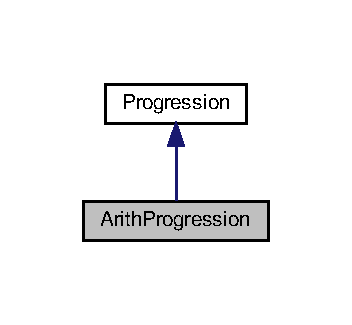
\includegraphics[width=169pt]{classArithProgression__inherit__graph}
\end{center}
\end{figure}


Collaboration diagram for Arith\+Progression\+:
\nopagebreak
\begin{figure}[H]
\begin{center}
\leavevmode
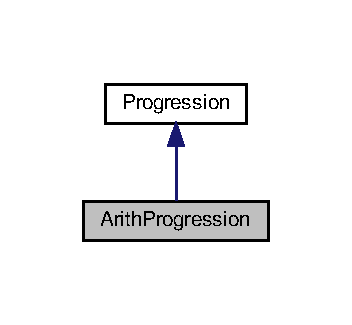
\includegraphics[width=169pt]{classArithProgression__coll__graph}
\end{center}
\end{figure}
\subsection*{Public Member Functions}
\begin{DoxyCompactItemize}
\item 
\mbox{\Hypertarget{classArithProgression_a6c3f2d78b0c158f05662b2ad7d48dec5}\label{classArithProgression_a6c3f2d78b0c158f05662b2ad7d48dec5}} 
{\bfseries Arith\+Progression} (long i=1)
\end{DoxyCompactItemize}
\subsection*{Protected Member Functions}
\begin{DoxyCompactItemize}
\item 
\mbox{\Hypertarget{classArithProgression_a257a52ae0e892ea0ed7fe29ff5b7577b}\label{classArithProgression_a257a52ae0e892ea0ed7fe29ff5b7577b}} 
virtual long {\bfseries next\+Value} ()
\end{DoxyCompactItemize}
\subsection*{Protected Attributes}
\begin{DoxyCompactItemize}
\item 
\mbox{\Hypertarget{classArithProgression_abe62e738f11278d06f2b7a642963a4cf}\label{classArithProgression_abe62e738f11278d06f2b7a642963a4cf}} 
long {\bfseries inc}
\end{DoxyCompactItemize}


The documentation for this class was generated from the following file\+:\begin{DoxyCompactItemize}
\item 
/home/oohnohnoh1/\+Desktop/\+G\+I\+T/\+Research/\+Parallel/include/openmp2.\+hpp\end{DoxyCompactItemize}

\hypertarget{classAudit}{}\section{Audit Class Reference}
\label{classAudit}\index{Audit@{Audit}}


Inheritance diagram for Audit\+:\nopagebreak
\begin{figure}[H]
\begin{center}
\leavevmode
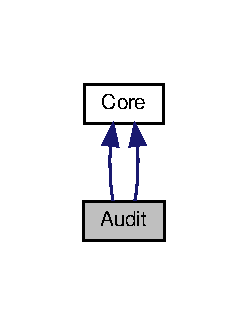
\includegraphics[width=119pt]{classAudit__inherit__graph}
\end{center}
\end{figure}


Collaboration diagram for Audit\+:\nopagebreak
\begin{figure}[H]
\begin{center}
\leavevmode
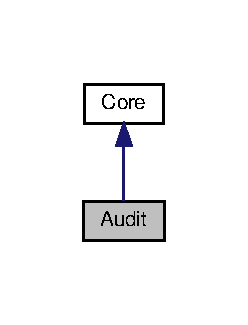
\includegraphics[width=121pt]{classAudit__coll__graph}
\end{center}
\end{figure}
\subsection*{Public Member Functions}
\begin{DoxyCompactItemize}
\item 
\mbox{\Hypertarget{classAudit_ade00f5809cf66ccdbcc9067e5b8a1fed}\label{classAudit_ade00f5809cf66ccdbcc9067e5b8a1fed}} 
{\bfseries Audit} (std\+::istream \&is)
\item 
\mbox{\Hypertarget{classAudit_a6919fff1539b7adbaf1f80162b873bd9}\label{classAudit_a6919fff1539b7adbaf1f80162b873bd9}} 
std\+::istream \& {\bfseries read} (std\+::istream \&)
\item 
\mbox{\Hypertarget{classAudit_a9e0ac89e1a2f1a36b3d37788ebec88f7}\label{classAudit_a9e0ac89e1a2f1a36b3d37788ebec88f7}} 
double {\bfseries grade} () const
\item 
\mbox{\Hypertarget{classAudit_a88378e2e72af376f5ff11ae5f41dfdfe}\label{classAudit_a88378e2e72af376f5ff11ae5f41dfdfe}} 
bool {\bfseries valid} () const
\item 
\mbox{\Hypertarget{classAudit_a3c9e02a58c0204f281c574fcd53cab55}\label{classAudit_a3c9e02a58c0204f281c574fcd53cab55}} 
bool {\bfseries fulfill\+\_\+reqs} () const
\item 
\mbox{\Hypertarget{classAudit_ade00f5809cf66ccdbcc9067e5b8a1fed}\label{classAudit_ade00f5809cf66ccdbcc9067e5b8a1fed}} 
{\bfseries Audit} (std\+::istream \&is)
\item 
\mbox{\Hypertarget{classAudit_a6919fff1539b7adbaf1f80162b873bd9}\label{classAudit_a6919fff1539b7adbaf1f80162b873bd9}} 
std\+::istream \& {\bfseries read} (std\+::istream \&)
\item 
\mbox{\Hypertarget{classAudit_a9e0ac89e1a2f1a36b3d37788ebec88f7}\label{classAudit_a9e0ac89e1a2f1a36b3d37788ebec88f7}} 
double {\bfseries grade} () const
\item 
\mbox{\Hypertarget{classAudit_a88378e2e72af376f5ff11ae5f41dfdfe}\label{classAudit_a88378e2e72af376f5ff11ae5f41dfdfe}} 
bool {\bfseries valid} () const
\item 
\mbox{\Hypertarget{classAudit_a3c9e02a58c0204f281c574fcd53cab55}\label{classAudit_a3c9e02a58c0204f281c574fcd53cab55}} 
bool {\bfseries fulfill\+\_\+reqs} () const
\end{DoxyCompactItemize}
\subsection*{Additional Inherited Members}


The documentation for this class was generated from the following files\+:\begin{DoxyCompactItemize}
\item 
/home/oohnohnoh1/\+Desktop/\+G\+I\+T/\+Research/\+Parallel/include/Core.\+h\item 
/home/oohnohnoh1/\+Desktop/\+G\+I\+T/\+Research/\+Parallel/include/openmp\+\_\+dynamicbindingandinheritance.\+hpp\end{DoxyCompactItemize}

\hypertarget{classbackground__task}{}\section{background\+\_\+task Class Reference}
\label{classbackground__task}\index{background\+\_\+task@{background\+\_\+task}}
\subsection*{Public Member Functions}
\begin{DoxyCompactItemize}
\item 
\mbox{\Hypertarget{classbackground__task_a116a774b35cf02ea68022f0be37f2ce9}\label{classbackground__task_a116a774b35cf02ea68022f0be37f2ce9}} 
void {\bfseries operator()} () const
\end{DoxyCompactItemize}


The documentation for this class was generated from the following file\+:\begin{DoxyCompactItemize}
\item 
/home/oohnohnoh1/\+Desktop/\+G\+I\+T/\+Research/\+Parallel/src/openmp\+\_\+thread.\+cxx\end{DoxyCompactItemize}

\hypertarget{classComplex}{}\section{Complex Class Reference}
\label{classComplex}\index{Complex@{Complex}}
\subsection*{Public Member Functions}
\begin{DoxyCompactItemize}
\item 
\mbox{\Hypertarget{classComplex_adee7e1752324bec9ae62ed2ce96b8ad3}\label{classComplex_adee7e1752324bec9ae62ed2ce96b8ad3}} 
{\bfseries Complex} (double r, double i=0)
\end{DoxyCompactItemize}
\subsection*{Friends}
\begin{DoxyCompactItemize}
\item 
\mbox{\Hypertarget{classComplex_a5a73e9d4e68af8cedb95bd0864054b89}\label{classComplex_a5a73e9d4e68af8cedb95bd0864054b89}} 
bool {\bfseries operator==} (const \hyperlink{classComplex}{Complex} \&a, const \hyperlink{classComplex}{Complex} \&b)
\end{DoxyCompactItemize}


The documentation for this class was generated from the following file\+:\begin{DoxyCompactItemize}
\item 
/home/oohnohnoh1/\+Desktop/\+G\+I\+T/\+Research/\+Parallel/src/openmp2.\+cxx\end{DoxyCompactItemize}

\hypertarget{classCore}{}\section{Core Class Reference}
\label{classCore}\index{Core@{Core}}


Inheritance diagram for Core\+:
\nopagebreak
\begin{figure}[H]
\begin{center}
\leavevmode
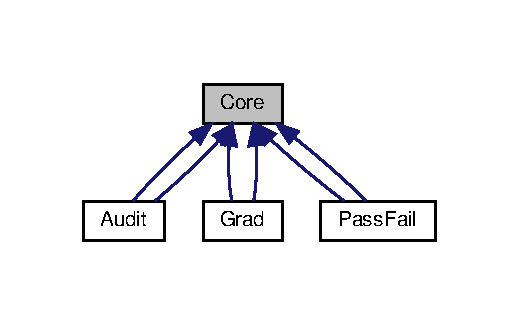
\includegraphics[width=249pt]{classCore__inherit__graph}
\end{center}
\end{figure}
\subsection*{Public Member Functions}
\begin{DoxyCompactItemize}
\item 
\mbox{\Hypertarget{classCore_ad1013e09510ddff40c114943de99093f}\label{classCore_ad1013e09510ddff40c114943de99093f}} 
{\bfseries Core} (std\+::istream \&is)
\item 
\mbox{\Hypertarget{classCore_a60d51fbac9805972bac7b117af8f1a54}\label{classCore_a60d51fbac9805972bac7b117af8f1a54}} 
std\+::string {\bfseries name} () const
\item 
\mbox{\Hypertarget{classCore_ae3bbc66cb3733082f8537d438c0521d6}\label{classCore_ae3bbc66cb3733082f8537d438c0521d6}} 
virtual std\+::istream \& {\bfseries read} (std\+::istream \&)
\item 
\mbox{\Hypertarget{classCore_a0d609cb4037c6dfe99ce0d68c1d69f04}\label{classCore_a0d609cb4037c6dfe99ce0d68c1d69f04}} 
virtual double {\bfseries grade} () const
\item 
\mbox{\Hypertarget{classCore_a557816073236f9ed9fa91edbb9cea451}\label{classCore_a557816073236f9ed9fa91edbb9cea451}} 
virtual bool {\bfseries valid} () const
\item 
\mbox{\Hypertarget{classCore_a81f50dc6932b75f6dbd7c9014bf23644}\label{classCore_a81f50dc6932b75f6dbd7c9014bf23644}} 
virtual bool {\bfseries fulfill\+\_\+reqs} () const
\end{DoxyCompactItemize}
\subsection*{Protected Member Functions}
\begin{DoxyCompactItemize}
\item 
\mbox{\Hypertarget{classCore_a05a303331fa92fae980dca24267a870e}\label{classCore_a05a303331fa92fae980dca24267a870e}} 
std\+::istream \& {\bfseries read\+\_\+common} (std\+::istream \&)
\item 
\mbox{\Hypertarget{classCore_ae781fdf236da68fabe00b8207608078b}\label{classCore_ae781fdf236da68fabe00b8207608078b}} 
virtual \hyperlink{classCore}{Core} $\ast$ {\bfseries clone} () const
\end{DoxyCompactItemize}
\subsection*{Protected Attributes}
\begin{DoxyCompactItemize}
\item 
\mbox{\Hypertarget{classCore_ac0329babd9f22f8858acbedb9e4346dc}\label{classCore_ac0329babd9f22f8858acbedb9e4346dc}} 
std\+::string {\bfseries n}
\item 
\mbox{\Hypertarget{classCore_a0af6c4fa1fe57bc1eb500d16dd546202}\label{classCore_a0af6c4fa1fe57bc1eb500d16dd546202}} 
double {\bfseries midterm}
\item 
\mbox{\Hypertarget{classCore_aa6cd0056b25e33c985fc8e347b9ed377}\label{classCore_aa6cd0056b25e33c985fc8e347b9ed377}} 
double {\bfseries final}
\item 
\mbox{\Hypertarget{classCore_a2975c3a0120d19df7bd74f40d518c3ef}\label{classCore_a2975c3a0120d19df7bd74f40d518c3ef}} 
std\+::vector$<$ double $>$ {\bfseries homework}
\end{DoxyCompactItemize}
\subsection*{Friends}
\begin{DoxyCompactItemize}
\item 
\mbox{\Hypertarget{classCore_a3697f82fec59c97d4afdca80e2f07686}\label{classCore_a3697f82fec59c97d4afdca80e2f07686}} 
class {\bfseries Student\+\_\+info}
\end{DoxyCompactItemize}


The documentation for this class was generated from the following files\+:\begin{DoxyCompactItemize}
\item 
/home/oohnohnoh1/\+Desktop/\+G\+I\+T/\+Research/\+Parallel/include/openmp\+\_\+dynamicbindingandinheritance.\+hpp\item 
/home/oohnohnoh1/\+Desktop/\+G\+I\+T/\+Research/\+Parallel/src/openmp\+\_\+dynamicbindingandinheritance.\+cxx\end{DoxyCompactItemize}

\hypertarget{classGrad}{}\section{Grad Class Reference}
\label{classGrad}\index{Grad@{Grad}}


Inheritance diagram for Grad\+:
\nopagebreak
\begin{figure}[H]
\begin{center}
\leavevmode
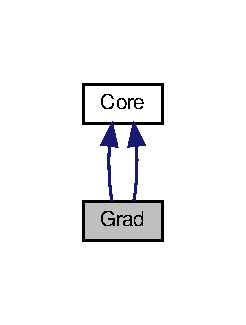
\includegraphics[width=118pt]{classGrad__inherit__graph}
\end{center}
\end{figure}


Collaboration diagram for Grad\+:
\nopagebreak
\begin{figure}[H]
\begin{center}
\leavevmode
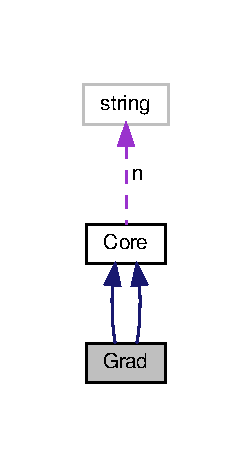
\includegraphics[width=118pt]{classGrad__coll__graph}
\end{center}
\end{figure}
\subsection*{Public Member Functions}
\begin{DoxyCompactItemize}
\item 
\mbox{\Hypertarget{classGrad_a683d203e0526d3926007681b7af7b0e5}\label{classGrad_a683d203e0526d3926007681b7af7b0e5}} 
{\bfseries Grad} (std\+::istream \&is)
\item 
\mbox{\Hypertarget{classGrad_ae3f9ebe99dfaa4ae86a87e457ae7a283}\label{classGrad_ae3f9ebe99dfaa4ae86a87e457ae7a283}} 
std\+::istream \& {\bfseries read} (std\+::istream \&)
\item 
\mbox{\Hypertarget{classGrad_aa481be2e8f7e4c16942221cd4931b431}\label{classGrad_aa481be2e8f7e4c16942221cd4931b431}} 
double {\bfseries grade} () const
\item 
\mbox{\Hypertarget{classGrad_ae2bae0e60fbce15836f55a90d0fc2c0e}\label{classGrad_ae2bae0e60fbce15836f55a90d0fc2c0e}} 
bool {\bfseries fulfill\+\_\+reqs} () const
\end{DoxyCompactItemize}
\subsection*{Additional Inherited Members}


The documentation for this class was generated from the following files\+:\begin{DoxyCompactItemize}
\item 
/home/oohnohnoh1/\+Desktop/\+G\+I\+T/\+Research/\+Parallel/include/openmp\+\_\+dynamicbindingandinheritance.\+hpp\item 
/home/oohnohnoh1/\+Desktop/\+G\+I\+T/\+Research/\+Parallel/src/openmp\+\_\+dynamicbindingandinheritance.\+cxx\end{DoxyCompactItemize}

\hypertarget{classInitiateVectorMethod}{}\section{Initiate\+Vector\+Method$<$ Item\+Type $>$ Class Template Reference}
\label{classInitiateVectorMethod}\index{Initiate\+Vector\+Method$<$ Item\+Type $>$@{Initiate\+Vector\+Method$<$ Item\+Type $>$}}
\subsection*{Public Member Functions}
\begin{DoxyCompactItemize}
\item 
\mbox{\Hypertarget{classInitiateVectorMethod_a9dd71b6c2afbb7d1dbccd86c5668df8d}\label{classInitiateVectorMethod_a9dd71b6c2afbb7d1dbccd86c5668df8d}} 
{\bfseries Initiate\+Vector\+Method} (int, int)
\item 
\mbox{\Hypertarget{classInitiateVectorMethod_ab3126dd49f59f317a9908fa1d86c4e5c}\label{classInitiateVectorMethod_ab3126dd49f59f317a9908fa1d86c4e5c}} 
void {\bfseries setup} (int $\ast$)
\item 
\mbox{\Hypertarget{classInitiateVectorMethod_a4cd80539ca03fc30bee98c9de786cbd8}\label{classInitiateVectorMethod_a4cd80539ca03fc30bee98c9de786cbd8}} 
void {\bfseries traits} ()
\item 
\mbox{\Hypertarget{classInitiateVectorMethod_aeefe1da73d131b57b36c8fcc25654683}\label{classInitiateVectorMethod_aeefe1da73d131b57b36c8fcc25654683}} 
void {\bfseries Send\+Vector} ()
\item 
\mbox{\Hypertarget{classInitiateVectorMethod_a0826022efb8056c18fe935be6675902b}\label{classInitiateVectorMethod_a0826022efb8056c18fe935be6675902b}} 
void {\bfseries Get\+Data} ()
\end{DoxyCompactItemize}


The documentation for this class was generated from the following file\+:\begin{DoxyCompactItemize}
\item 
/home/oohnohnoh1/\+Desktop/\+G\+I\+T/\+Research/\+Parallel/include/new.\+hpp\end{DoxyCompactItemize}

\hypertarget{classMPI__BC}{}\section{M\+P\+I\+\_\+\+BC Class Reference}
\label{classMPI__BC}\index{M\+P\+I\+\_\+\+BC@{M\+P\+I\+\_\+\+BC}}


Inheritance diagram for M\+P\+I\+\_\+\+BC\+:\nopagebreak
\begin{figure}[H]
\begin{center}
\leavevmode
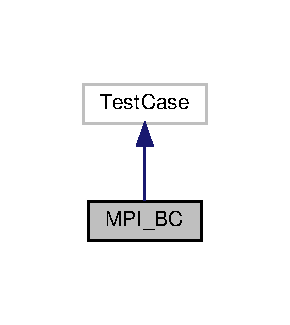
\includegraphics[width=139pt]{classMPI__BC__inherit__graph}
\end{center}
\end{figure}


Collaboration diagram for M\+P\+I\+\_\+\+BC\+:\nopagebreak
\begin{figure}[H]
\begin{center}
\leavevmode
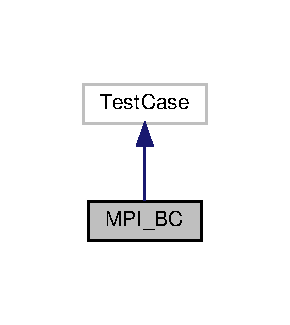
\includegraphics[width=139pt]{classMPI__BC__coll__graph}
\end{center}
\end{figure}
\subsection*{Public Member Functions}
\begin{DoxyCompactItemize}
\item 
\hyperlink{classMPI__BC_a1c761fcc4df7e6809a0ffd2a20cebd12}{M\+P\+I\+\_\+\+BC} ()
\begin{DoxyCompactList}\small\item\em \hyperlink{classMPI__BC}{M\+P\+I\+\_\+\+BC} class template filling. \end{DoxyCompactList}\item 
\mbox{\Hypertarget{classMPI__BC_ae489483851e7b20c09ffe112e514f25c}\label{classMPI__BC_ae489483851e7b20c09ffe112e514f25c}} 
void {\bfseries pack\+Data} ()
\item 
\mbox{\Hypertarget{classMPI__BC_a833339bd5f16e9d09c1ae15f2870c175}\label{classMPI__BC_a833339bd5f16e9d09c1ae15f2870c175}} 
void {\bfseries time\+\_\+ellapsed} ()
\item 
\mbox{\Hypertarget{classMPI__BC_a336da02d01deace3059d280a5d797d46}\label{classMPI__BC_a336da02d01deace3059d280a5d797d46}} 
void {\bfseries broadcast\+\_\+input} ()
\item 
\mbox{\Hypertarget{classMPI__BC_a71eb5c66f0072f0c55c8975898eb8edb}\label{classMPI__BC_a71eb5c66f0072f0c55c8975898eb8edb}} 
void {\bfseries broadcast\+\_\+vector} ()
\item 
\mbox{\Hypertarget{classMPI__BC_a040c0384ca72ca971eeea94a7e90aa05}\label{classMPI__BC_a040c0384ca72ca971eeea94a7e90aa05}} 
void {\bfseries build\+Mpi\+Type} (double $\ast$, double $\ast$, int $\ast$, M\+P\+I\+\_\+\+Datatype $\ast$)
\item 
\mbox{\Hypertarget{classMPI__BC_a2134566ddece0822a5e3714b3ec13c20}\label{classMPI__BC_a2134566ddece0822a5e3714b3ec13c20}} 
void {\bfseries Send} (float, float, int, int)
\item 
\mbox{\Hypertarget{classMPI__BC_ada7b741145acc727755fa5dfabbc9575}\label{classMPI__BC_ada7b741145acc727755fa5dfabbc9575}} 
void {\bfseries Send\+Vector} ()
\item 
\mbox{\Hypertarget{classMPI__BC_a64ce44132cb41a0cd45ac15601bba6a2}\label{classMPI__BC_a64ce44132cb41a0cd45ac15601bba6a2}} 
void {\bfseries Receive} (float $\ast$, float $\ast$, int $\ast$, int)
\item 
\mbox{\Hypertarget{classMPI__BC_a7bfcbf6d2b35ef6894dca53ac4b14af1}\label{classMPI__BC_a7bfcbf6d2b35ef6894dca53ac4b14af1}} 
void {\bfseries parallel\+Allocate\+Vec} (double $\ast$, double $\ast$, int, std\+::vector$<$ int $>$ $\ast$, M\+P\+I\+\_\+\+Datatype $\ast$)
\end{DoxyCompactItemize}


\subsection{Constructor \& Destructor Documentation}
\mbox{\Hypertarget{classMPI__BC_a1c761fcc4df7e6809a0ffd2a20cebd12}\label{classMPI__BC_a1c761fcc4df7e6809a0ffd2a20cebd12}} 
\index{M\+P\+I\+\_\+\+BC@{M\+P\+I\+\_\+\+BC}!M\+P\+I\+\_\+\+BC@{M\+P\+I\+\_\+\+BC}}
\index{M\+P\+I\+\_\+\+BC@{M\+P\+I\+\_\+\+BC}!M\+P\+I\+\_\+\+BC@{M\+P\+I\+\_\+\+BC}}
\subsubsection{\texorpdfstring{M\+P\+I\+\_\+\+B\+C()}{MPI\_BC()}}
{\footnotesize\ttfamily M\+P\+I\+\_\+\+B\+C\+::\+M\+P\+I\+\_\+\+BC (\begin{DoxyParamCaption}{ }\end{DoxyParamCaption})}



\hyperlink{classMPI__BC}{M\+P\+I\+\_\+\+BC} class template filling. 

Placeholder 

The documentation for this class was generated from the following files\+:\begin{DoxyCompactItemize}
\item 
/home/oohnohnoh1/\+Desktop/\+G\+I\+T/\+Research/\+Parallel/include/M\+P\+I\+\_\+broadcast.\+hpp\item 
/home/oohnohnoh1/\+Desktop/\+G\+I\+T/\+Research/\+Parallel/src/M\+P\+I\+\_\+broadcast.\+cxx\end{DoxyCompactItemize}

\hypertarget{classMPI__BC__Generic}{}\section{M\+P\+I\+\_\+\+B\+C\+\_\+\+Generic$<$ T, Q, R $>$ Class Template Reference}
\label{classMPI__BC__Generic}\index{M\+P\+I\+\_\+\+B\+C\+\_\+\+Generic$<$ T, Q, R $>$@{M\+P\+I\+\_\+\+B\+C\+\_\+\+Generic$<$ T, Q, R $>$}}
\subsection*{Public Member Functions}
\begin{DoxyCompactItemize}
\item 
\mbox{\Hypertarget{classMPI__BC__Generic_a5259faca161859023e33e2e622f0a89b}\label{classMPI__BC__Generic_a5259faca161859023e33e2e622f0a89b}} 
{\bfseries M\+P\+I\+\_\+\+B\+C\+\_\+\+Generic} (std\+::size\+\_\+t n)
\end{DoxyCompactItemize}


The documentation for this class was generated from the following file\+:\begin{DoxyCompactItemize}
\item 
/home/oohnohnoh1/\+Desktop/\+G\+I\+T/\+Research/\+Parallel/include/M\+P\+I\+\_\+broadcast.\+hpp\end{DoxyCompactItemize}

\hypertarget{classMPI__sorting__methods}{}\section{M\+P\+I\+\_\+sorting\+\_\+methods Class Reference}
\label{classMPI__sorting__methods}\index{M\+P\+I\+\_\+sorting\+\_\+methods@{M\+P\+I\+\_\+sorting\+\_\+methods}}
\subsection*{Public Member Functions}
\begin{DoxyCompactItemize}
\item 
\mbox{\Hypertarget{classMPI__sorting__methods_a1cd738d8c9e6817b98680d4243d8d3c5}\label{classMPI__sorting__methods_a1cd738d8c9e6817b98680d4243d8d3c5}} 
void {\bfseries Bubble\+\_\+sort} (int a\mbox{[}$\,$\mbox{]}, int n)
\end{DoxyCompactItemize}


The documentation for this class was generated from the following file\+:\begin{DoxyCompactItemize}
\item 
/home/oohnohnoh1/\+Desktop/\+G\+I\+T/\+Research/\+Parallel/src/M\+P\+I\+\_\+reduce.\+cxx\end{DoxyCompactItemize}

\hypertarget{classMPIInput}{}\section{M\+P\+I\+Input Class Reference}
\label{classMPIInput}\index{M\+P\+I\+Input@{M\+P\+I\+Input}}
\subsection*{Public Member Functions}
\begin{DoxyCompactItemize}
\item 
\hyperlink{classMPIInput_a1fd40b314f5e63f0948050dd687f2d6d}{M\+P\+I\+Input} ()
\begin{DoxyCompactList}\small\item\em \hyperlink{classMPIInput}{M\+P\+I\+Input} class -\/ constructor. \end{DoxyCompactList}\item 
\hyperlink{classMPIInput_aad9097968754daede74b4e9931f58c8a}{M\+P\+I\+Input} (int, int)
\begin{DoxyCompactList}\small\item\em \hyperlink{classMPIInput}{M\+P\+I\+Input} class -\/ constructor. \end{DoxyCompactList}\item 
void \hyperlink{classMPIInput_a5204b6d3bea6d1d6110b6d180da43e07}{M\+P\+I\+Start} ()
\begin{DoxyCompactList}\small\item\em \hyperlink{classMPIInput}{M\+P\+I\+Input} class -\/ M\+P\+I\+Start method. \end{DoxyCompactList}\item 
void \hyperlink{classMPIInput_ab573f01916c4e35072009b95602a1399}{get\+Data} ()
\item 
\mbox{\Hypertarget{classMPIInput_a03c8faee4d48167f2ab33b52fad7e5ea}\label{classMPIInput_a03c8faee4d48167f2ab33b52fad7e5ea}} 
void {\bfseries bubble\+Sort} ()
\item 
\mbox{\Hypertarget{classMPIInput_a1c6165f90d30a3988eba3b9cea5afefa}\label{classMPIInput_a1c6165f90d30a3988eba3b9cea5afefa}} 
void {\bfseries odd\+Even\+Sort} ()
\item 
\mbox{\Hypertarget{classMPIInput_ab90ddedf8faad1bfeb850d6303af50a5}\label{classMPIInput_ab90ddedf8faad1bfeb850d6303af50a5}} 
void {\bfseries I\+\_\+send} ()
\end{DoxyCompactItemize}


\subsection{Constructor \& Destructor Documentation}
\mbox{\Hypertarget{classMPIInput_a1fd40b314f5e63f0948050dd687f2d6d}\label{classMPIInput_a1fd40b314f5e63f0948050dd687f2d6d}} 
\index{M\+P\+I\+Input@{M\+P\+I\+Input}!M\+P\+I\+Input@{M\+P\+I\+Input}}
\index{M\+P\+I\+Input@{M\+P\+I\+Input}!M\+P\+I\+Input@{M\+P\+I\+Input}}
\subsubsection{\texorpdfstring{M\+P\+I\+Input()}{MPIInput()}\hspace{0.1cm}{\footnotesize\ttfamily [1/2]}}
{\footnotesize\ttfamily M\+P\+I\+Input\+::\+M\+P\+I\+Input (\begin{DoxyParamCaption}{ }\end{DoxyParamCaption})}



\hyperlink{classMPIInput}{M\+P\+I\+Input} class -\/ constructor. 

Default constructor

The default constructor \mbox{\Hypertarget{classMPIInput_aad9097968754daede74b4e9931f58c8a}\label{classMPIInput_aad9097968754daede74b4e9931f58c8a}} 
\index{M\+P\+I\+Input@{M\+P\+I\+Input}!M\+P\+I\+Input@{M\+P\+I\+Input}}
\index{M\+P\+I\+Input@{M\+P\+I\+Input}!M\+P\+I\+Input@{M\+P\+I\+Input}}
\subsubsection{\texorpdfstring{M\+P\+I\+Input()}{MPIInput()}\hspace{0.1cm}{\footnotesize\ttfamily [2/2]}}
{\footnotesize\ttfamily M\+P\+I\+Input\+::\+M\+P\+I\+Input (\begin{DoxyParamCaption}\item[{int}]{mr,  }\item[{int}]{pe }\end{DoxyParamCaption})}



\hyperlink{classMPIInput}{M\+P\+I\+Input} class -\/ constructor. 

int int constructor

The input constructor 

\subsection{Member Function Documentation}
\mbox{\Hypertarget{classMPIInput_ab573f01916c4e35072009b95602a1399}\label{classMPIInput_ab573f01916c4e35072009b95602a1399}} 
\index{M\+P\+I\+Input@{M\+P\+I\+Input}!get\+Data@{get\+Data}}
\index{get\+Data@{get\+Data}!M\+P\+I\+Input@{M\+P\+I\+Input}}
\subsubsection{\texorpdfstring{get\+Data()}{getData()}}
{\footnotesize\ttfamily void M\+P\+I\+Input\+::get\+Data (\begin{DoxyParamCaption}{ }\end{DoxyParamCaption})}

M\+P\+I\+\_\+pack allows ..\mbox{\Hypertarget{classMPIInput_a5204b6d3bea6d1d6110b6d180da43e07}\label{classMPIInput_a5204b6d3bea6d1d6110b6d180da43e07}} 
\index{M\+P\+I\+Input@{M\+P\+I\+Input}!M\+P\+I\+Start@{M\+P\+I\+Start}}
\index{M\+P\+I\+Start@{M\+P\+I\+Start}!M\+P\+I\+Input@{M\+P\+I\+Input}}
\subsubsection{\texorpdfstring{M\+P\+I\+Start()}{MPIStart()}}
{\footnotesize\ttfamily void M\+P\+I\+Input\+::\+M\+P\+I\+Start (\begin{DoxyParamCaption}{ }\end{DoxyParamCaption})}



\hyperlink{classMPIInput}{M\+P\+I\+Input} class -\/ M\+P\+I\+Start method. 

Sets up the processor ranks and size for use later -\/ could really be incoporated into the consturcotr 

The documentation for this class was generated from the following files\+:\begin{DoxyCompactItemize}
\item 
/home/oohnohnoh1/\+Desktop/\+G\+I\+T/\+Research/\+Parallel/include/M\+P\+I\+\_\+\+I\+O.\+hpp\item 
/home/oohnohnoh1/\+Desktop/\+G\+I\+T/\+Research/\+Parallel/src/M\+P\+I\+\_\+\+I\+O.\+cxx\end{DoxyCompactItemize}

\hypertarget{classOMP}{}\section{O\+MP$<$ T $>$ Class Template Reference}
\label{classOMP}\index{O\+M\+P$<$ T $>$@{O\+M\+P$<$ T $>$}}
\subsection*{Public Member Functions}
\begin{DoxyCompactItemize}
\item 
\mbox{\Hypertarget{classOMP_aa2d683844b0c792f2e4b8004282c3c4f}\label{classOMP_aa2d683844b0c792f2e4b8004282c3c4f}} 
{\bfseries O\+MP} (int)
\item 
\mbox{\Hypertarget{classOMP_a74734b9e39249242a4d81c4c843a8497}\label{classOMP_a74734b9e39249242a4d81c4c843a8497}} 
{\bfseries O\+MP} (const \hyperlink{classOMP}{O\+MP} \&O\+M\+P\+Copy)
\item 
\mbox{\Hypertarget{classOMP_a8e5d794021f25dc36d486d0a268d7713}\label{classOMP_a8e5d794021f25dc36d486d0a268d7713}} 
\hyperlink{classOMP}{O\+MP} \& {\bfseries operator=} (const \hyperlink{classOMP}{O\+MP} \&ref)
\item 
\mbox{\Hypertarget{classOMP_a4d9450a0c0304e2cd2d705ca06e450cc}\label{classOMP_a4d9450a0c0304e2cd2d705ca06e450cc}} 
void {\bfseries add} (T)
\item 
\mbox{\Hypertarget{classOMP_a315d43939578681fd9ffc52259e81996}\label{classOMP_a315d43939578681fd9ffc52259e81996}} 
void {\bfseries addup} ()
\item 
\mbox{\Hypertarget{classOMP_af2e1072e3c0bf76fd14379eeca69dff9}\label{classOMP_af2e1072e3c0bf76fd14379eeca69dff9}} 
void {\bfseries pi} ()
\end{DoxyCompactItemize}


The documentation for this class was generated from the following file\+:\begin{DoxyCompactItemize}
\item 
/home/oohnohnoh1/\+Desktop/\+G\+I\+T/\+Research/\+Parallel/include/openmp1.\+hpp\end{DoxyCompactItemize}

\hypertarget{structPartstruct}{}\section{Partstruct Struct Reference}
\label{structPartstruct}\index{Partstruct@{Partstruct}}
\subsection*{Public Attributes}
\begin{DoxyCompactItemize}
\item 
\mbox{\Hypertarget{structPartstruct_a62ad380a974f632c6d75171ea1f4b7d2}\label{structPartstruct_a62ad380a974f632c6d75171ea1f4b7d2}} 
int {\bfseries class}
\item 
\mbox{\Hypertarget{structPartstruct_ad110813138b77734d28a81bc344033aa}\label{structPartstruct_ad110813138b77734d28a81bc344033aa}} 
double {\bfseries d} \mbox{[}6\mbox{]}
\item 
\mbox{\Hypertarget{structPartstruct_ae19dcf24189bec433d17fe6b22669e9e}\label{structPartstruct_ae19dcf24189bec433d17fe6b22669e9e}} 
char {\bfseries b} \mbox{[}7\mbox{]}
\end{DoxyCompactItemize}


The documentation for this struct was generated from the following file\+:\begin{DoxyCompactItemize}
\item 
/home/oohnohnoh1/\+Desktop/\+G\+I\+T/\+Research/\+Parallel/src/M\+P\+I\+\_\+struct.\+cxx\end{DoxyCompactItemize}

\hypertarget{classPassFail}{}\section{Pass\+Fail Class Reference}
\label{classPassFail}\index{Pass\+Fail@{Pass\+Fail}}


Inheritance diagram for Pass\+Fail\+:\nopagebreak
\begin{figure}[H]
\begin{center}
\leavevmode
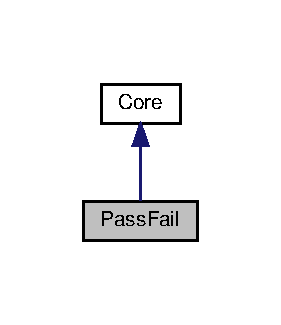
\includegraphics[width=135pt]{classPassFail__inherit__graph}
\end{center}
\end{figure}


Collaboration diagram for Pass\+Fail\+:\nopagebreak
\begin{figure}[H]
\begin{center}
\leavevmode
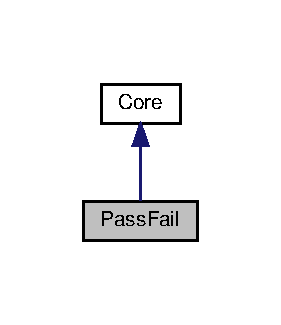
\includegraphics[width=135pt]{classPassFail__coll__graph}
\end{center}
\end{figure}
\subsection*{Public Member Functions}
\begin{DoxyCompactItemize}
\item 
\mbox{\Hypertarget{classPassFail_a5c90795505aa60da716935c450919b77}\label{classPassFail_a5c90795505aa60da716935c450919b77}} 
{\bfseries Pass\+Fail} (std\+::istream \&is)
\item 
\mbox{\Hypertarget{classPassFail_a7f96a2d51a1a72c131ee93aa53bd5848}\label{classPassFail_a7f96a2d51a1a72c131ee93aa53bd5848}} 
double {\bfseries grade} () const
\item 
\mbox{\Hypertarget{classPassFail_a06c77d7cd3c48f95476c17c53a6d7e7c}\label{classPassFail_a06c77d7cd3c48f95476c17c53a6d7e7c}} 
bool {\bfseries valid} () const
\item 
\mbox{\Hypertarget{classPassFail_a46d15c8f5f28b4c7b8f1311745c9a2a5}\label{classPassFail_a46d15c8f5f28b4c7b8f1311745c9a2a5}} 
bool {\bfseries fulfill\+\_\+reqs} () const
\item 
\mbox{\Hypertarget{classPassFail_a5c90795505aa60da716935c450919b77}\label{classPassFail_a5c90795505aa60da716935c450919b77}} 
{\bfseries Pass\+Fail} (std\+::istream \&is)
\item 
\mbox{\Hypertarget{classPassFail_a7f96a2d51a1a72c131ee93aa53bd5848}\label{classPassFail_a7f96a2d51a1a72c131ee93aa53bd5848}} 
double {\bfseries grade} () const
\item 
\mbox{\Hypertarget{classPassFail_a06c77d7cd3c48f95476c17c53a6d7e7c}\label{classPassFail_a06c77d7cd3c48f95476c17c53a6d7e7c}} 
bool {\bfseries valid} () const
\item 
\mbox{\Hypertarget{classPassFail_a46d15c8f5f28b4c7b8f1311745c9a2a5}\label{classPassFail_a46d15c8f5f28b4c7b8f1311745c9a2a5}} 
bool {\bfseries fulfill\+\_\+reqs} () const
\end{DoxyCompactItemize}
\subsection*{Additional Inherited Members}


The documentation for this class was generated from the following files\+:\begin{DoxyCompactItemize}
\item 
/home/oohnohnoh1/\+Desktop/\+G\+I\+T/\+Research/\+Parallel/include/Core.\+h\item 
/home/oohnohnoh1/\+Desktop/\+G\+I\+T/\+Research/\+Parallel/include/openmp\+\_\+dynamicbindingandinheritance.\+hpp\end{DoxyCompactItemize}

\hypertarget{classpart1_1_1Point}{}\section{part1\+:\+:Point Class Reference}
\label{classpart1_1_1Point}\index{part1\+::\+Point@{part1\+::\+Point}}


{\ttfamily \#include $<$lib\+\_\+mpi.\+hpp$>$}

\subsection*{Public Member Functions}
\begin{DoxyCompactItemize}
\item 
\mbox{\Hypertarget{classpart1_1_1Point_a483975ffea2151c9b12890c086bcbcc6}\label{classpart1_1_1Point_a483975ffea2151c9b12890c086bcbcc6}} 
{\bfseries Point} (float \+\_\+x, float \+\_\+y, float \+\_\+z)
\end{DoxyCompactItemize}
\subsection*{Public Attributes}
\begin{DoxyCompactItemize}
\item 
\mbox{\Hypertarget{classpart1_1_1Point_a179479d169ee6cedc42c61aaaa51935e}\label{classpart1_1_1Point_a179479d169ee6cedc42c61aaaa51935e}} 
float {\bfseries x}
\item 
\mbox{\Hypertarget{classpart1_1_1Point_a8842e404aca1f960a1ab7d9bcffc16cf}\label{classpart1_1_1Point_a8842e404aca1f960a1ab7d9bcffc16cf}} 
float {\bfseries y}
\item 
\mbox{\Hypertarget{classpart1_1_1Point_a246edeeae578e2d733be9d888c59b980}\label{classpart1_1_1Point_a246edeeae578e2d733be9d888c59b980}} 
float {\bfseries z}
\end{DoxyCompactItemize}


\subsection{Detailed Description}
This is a simple 3D point class 

The documentation for this class was generated from the following file\+:\begin{DoxyCompactItemize}
\item 
/home/oohnohnoh1/\+Desktop/\+G\+I\+T/\+Research/\+Parallel/include/lib\+\_\+mpi.\+hpp\end{DoxyCompactItemize}

\hypertarget{classProgression}{}\section{Progression Class Reference}
\label{classProgression}\index{Progression@{Progression}}


Inheritance diagram for Progression\+:\nopagebreak
\begin{figure}[H]
\begin{center}
\leavevmode
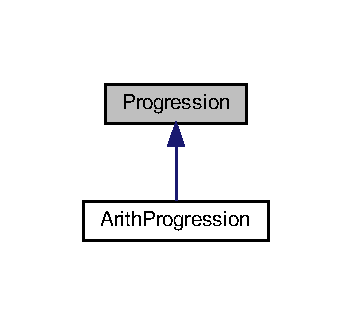
\includegraphics[width=169pt]{classProgression__inherit__graph}
\end{center}
\end{figure}
\subsection*{Public Member Functions}
\begin{DoxyCompactItemize}
\item 
\mbox{\Hypertarget{classProgression_a4d746d05334214c18f8cda8ff6006659}\label{classProgression_a4d746d05334214c18f8cda8ff6006659}} 
{\bfseries Progression} (long f=0)
\item 
\mbox{\Hypertarget{classProgression_ad652f1d934da13b088422f675212e1fd}\label{classProgression_ad652f1d934da13b088422f675212e1fd}} 
void {\bfseries print\+Progression} (int n)
\end{DoxyCompactItemize}
\subsection*{Protected Member Functions}
\begin{DoxyCompactItemize}
\item 
\mbox{\Hypertarget{classProgression_aa930e887ec5fc8ba27c358e43d561393}\label{classProgression_aa930e887ec5fc8ba27c358e43d561393}} 
virtual long {\bfseries first\+Value} ()
\item 
\mbox{\Hypertarget{classProgression_a52e78526540e4e1f1194a2936160e9a4}\label{classProgression_a52e78526540e4e1f1194a2936160e9a4}} 
virtual long {\bfseries next\+Value} ()
\end{DoxyCompactItemize}
\subsection*{Protected Attributes}
\begin{DoxyCompactItemize}
\item 
\mbox{\Hypertarget{classProgression_a3846cba453b88d1ea89d94c41d7a6fe3}\label{classProgression_a3846cba453b88d1ea89d94c41d7a6fe3}} 
long {\bfseries first}
\item 
\mbox{\Hypertarget{classProgression_ab1794ef4de7de380bda5e9c09a785126}\label{classProgression_ab1794ef4de7de380bda5e9c09a785126}} 
long {\bfseries cur}
\end{DoxyCompactItemize}


The documentation for this class was generated from the following file\+:\begin{DoxyCompactItemize}
\item 
/home/oohnohnoh1/\+Desktop/\+G\+I\+T/\+Research/\+Parallel/include/openmp2.\+hpp\end{DoxyCompactItemize}

\hypertarget{classQTstyle__Test}{}\section{Q\+Tstyle\+\_\+\+Test Class Reference}
\label{classQTstyle__Test}\index{Q\+Tstyle\+\_\+\+Test@{Q\+Tstyle\+\_\+\+Test}}


A test class.  




{\ttfamily \#include $<$J\+E\+\_\+compute.\+hpp$>$}

\subsection*{Public Types}
\begin{DoxyCompactItemize}
\item 
enum \hyperlink{classQTstyle__Test_a0525f798cda415a94fedeceb806d2c49}{T\+Enum} \{ \hyperlink{classQTstyle__Test_a0525f798cda415a94fedeceb806d2c49a7929af91f99c319ffe2e49c9632bc3fa}{T\+Val1}, 
\hyperlink{classQTstyle__Test_a0525f798cda415a94fedeceb806d2c49afff89db6859123549579806212d9fd80}{T\+Val2}, 
\hyperlink{classQTstyle__Test_a0525f798cda415a94fedeceb806d2c49a8227cd0f0c1285d59ff14376fcd00f85}{T\+Val3}
 \}\begin{DoxyCompactList}\small\item\em An enum. \end{DoxyCompactList}
\end{DoxyCompactItemize}
\subsection*{Public Member Functions}
\begin{DoxyCompactItemize}
\item 
\hyperlink{classQTstyle__Test_a14a296ea4e2ad446712f2310bec60766}{Q\+Tstyle\+\_\+\+Test} ()
\begin{DoxyCompactList}\small\item\em A constructor. \end{DoxyCompactList}\item 
\hyperlink{classQTstyle__Test_a7e82397d534d9a867f0857da01a46e9e}{$\sim$\+Q\+Tstyle\+\_\+\+Test} ()
\begin{DoxyCompactList}\small\item\em A destructor. \end{DoxyCompactList}\item 
int \hyperlink{classQTstyle__Test_a8840748753118dd468e8368a28e49c62}{test\+Me} (int a, const char $\ast$s)
\begin{DoxyCompactList}\small\item\em A normal member taking two arguments and returning an integer value. \end{DoxyCompactList}\item 
virtual void \hyperlink{classQTstyle__Test_ad5b201f097a720d44bf976c2f27efbda}{test\+Me\+Too} (char c1, char c2)=0
\begin{DoxyCompactList}\small\item\em A pure virtual member. \end{DoxyCompactList}\end{DoxyCompactItemize}
\subsection*{Public Attributes}
\begin{DoxyCompactItemize}
\item 
enum \hyperlink{classQTstyle__Test_a0525f798cda415a94fedeceb806d2c49}{Q\+Tstyle\+\_\+\+Test\+::\+T\+Enum} $\ast$ \hyperlink{classQTstyle__Test_a973a4566c9a036f4eca508ba5fe80dcb}{enum\+Ptr}
\begin{DoxyCompactList}\small\item\em Enum pointer. \end{DoxyCompactList}\item 
enum \hyperlink{classQTstyle__Test_a0525f798cda415a94fedeceb806d2c49}{Q\+Tstyle\+\_\+\+Test\+::\+T\+Enum} \hyperlink{classQTstyle__Test_adb265d815b43f1f7f0de0e8b8852a5d0}{enum\+Var}
\begin{DoxyCompactList}\small\item\em Enum variable. \end{DoxyCompactList}\item 
int \hyperlink{classQTstyle__Test_aabf7b2e9ed83ea44aca4d213baae06d3}{public\+Var}
\begin{DoxyCompactList}\small\item\em A public variable. \end{DoxyCompactList}\item 
int($\ast$ \hyperlink{classQTstyle__Test_a79dd4e5498f09057775a819d911349e2}{handler} )(int a, int b)
\begin{DoxyCompactList}\small\item\em A function variable. \end{DoxyCompactList}\end{DoxyCompactItemize}


\subsection{Detailed Description}
A test class. 

A more elaborate class description. 

\subsection{Member Enumeration Documentation}
\mbox{\Hypertarget{classQTstyle__Test_a0525f798cda415a94fedeceb806d2c49}\label{classQTstyle__Test_a0525f798cda415a94fedeceb806d2c49}} 
\index{Q\+Tstyle\+\_\+\+Test@{Q\+Tstyle\+\_\+\+Test}!T\+Enum@{T\+Enum}}
\index{T\+Enum@{T\+Enum}!Q\+Tstyle\+\_\+\+Test@{Q\+Tstyle\+\_\+\+Test}}
\subsubsection{\texorpdfstring{T\+Enum}{TEnum}}
{\footnotesize\ttfamily enum \hyperlink{classQTstyle__Test_a0525f798cda415a94fedeceb806d2c49}{Q\+Tstyle\+\_\+\+Test\+::\+T\+Enum}}



An enum. 

More detailed enum description. \begin{DoxyEnumFields}{Enumerator}
\raisebox{\heightof{T}}[0pt][0pt]{\index{T\+Val1@{T\+Val1}!Q\+Tstyle\+\_\+\+Test@{Q\+Tstyle\+\_\+\+Test}}\index{Q\+Tstyle\+\_\+\+Test@{Q\+Tstyle\+\_\+\+Test}!T\+Val1@{T\+Val1}}}\mbox{\Hypertarget{classQTstyle__Test_a0525f798cda415a94fedeceb806d2c49a7929af91f99c319ffe2e49c9632bc3fa}\label{classQTstyle__Test_a0525f798cda415a94fedeceb806d2c49a7929af91f99c319ffe2e49c9632bc3fa}} 
T\+Val1&Enum value T\+Val1. \\
\hline

\raisebox{\heightof{T}}[0pt][0pt]{\index{T\+Val2@{T\+Val2}!Q\+Tstyle\+\_\+\+Test@{Q\+Tstyle\+\_\+\+Test}}\index{Q\+Tstyle\+\_\+\+Test@{Q\+Tstyle\+\_\+\+Test}!T\+Val2@{T\+Val2}}}\mbox{\Hypertarget{classQTstyle__Test_a0525f798cda415a94fedeceb806d2c49afff89db6859123549579806212d9fd80}\label{classQTstyle__Test_a0525f798cda415a94fedeceb806d2c49afff89db6859123549579806212d9fd80}} 
T\+Val2&Enum value T\+Val2. \\
\hline

\raisebox{\heightof{T}}[0pt][0pt]{\index{T\+Val3@{T\+Val3}!Q\+Tstyle\+\_\+\+Test@{Q\+Tstyle\+\_\+\+Test}}\index{Q\+Tstyle\+\_\+\+Test@{Q\+Tstyle\+\_\+\+Test}!T\+Val3@{T\+Val3}}}\mbox{\Hypertarget{classQTstyle__Test_a0525f798cda415a94fedeceb806d2c49a8227cd0f0c1285d59ff14376fcd00f85}\label{classQTstyle__Test_a0525f798cda415a94fedeceb806d2c49a8227cd0f0c1285d59ff14376fcd00f85}} 
T\+Val3&Enum value T\+Val3. \\
\hline

\end{DoxyEnumFields}


\subsection{Constructor \& Destructor Documentation}
\mbox{\Hypertarget{classQTstyle__Test_a14a296ea4e2ad446712f2310bec60766}\label{classQTstyle__Test_a14a296ea4e2ad446712f2310bec60766}} 
\index{Q\+Tstyle\+\_\+\+Test@{Q\+Tstyle\+\_\+\+Test}!Q\+Tstyle\+\_\+\+Test@{Q\+Tstyle\+\_\+\+Test}}
\index{Q\+Tstyle\+\_\+\+Test@{Q\+Tstyle\+\_\+\+Test}!Q\+Tstyle\+\_\+\+Test@{Q\+Tstyle\+\_\+\+Test}}
\subsubsection{\texorpdfstring{Q\+Tstyle\+\_\+\+Test()}{QTstyle\_Test()}}
{\footnotesize\ttfamily Q\+Tstyle\+\_\+\+Test\+::\+Q\+Tstyle\+\_\+\+Test (\begin{DoxyParamCaption}{ }\end{DoxyParamCaption})}



A constructor. 

A more elaborate description of the constructor. \mbox{\Hypertarget{classQTstyle__Test_a7e82397d534d9a867f0857da01a46e9e}\label{classQTstyle__Test_a7e82397d534d9a867f0857da01a46e9e}} 
\index{Q\+Tstyle\+\_\+\+Test@{Q\+Tstyle\+\_\+\+Test}!````~Q\+Tstyle\+\_\+\+Test@{$\sim$\+Q\+Tstyle\+\_\+\+Test}}
\index{````~Q\+Tstyle\+\_\+\+Test@{$\sim$\+Q\+Tstyle\+\_\+\+Test}!Q\+Tstyle\+\_\+\+Test@{Q\+Tstyle\+\_\+\+Test}}
\subsubsection{\texorpdfstring{$\sim$\+Q\+Tstyle\+\_\+\+Test()}{~QTstyle\_Test()}}
{\footnotesize\ttfamily Q\+Tstyle\+\_\+\+Test\+::$\sim$\+Q\+Tstyle\+\_\+\+Test (\begin{DoxyParamCaption}{ }\end{DoxyParamCaption})}



A destructor. 

A more elaborate description of the destructor. 

\subsection{Member Function Documentation}
\mbox{\Hypertarget{classQTstyle__Test_a8840748753118dd468e8368a28e49c62}\label{classQTstyle__Test_a8840748753118dd468e8368a28e49c62}} 
\index{Q\+Tstyle\+\_\+\+Test@{Q\+Tstyle\+\_\+\+Test}!test\+Me@{test\+Me}}
\index{test\+Me@{test\+Me}!Q\+Tstyle\+\_\+\+Test@{Q\+Tstyle\+\_\+\+Test}}
\subsubsection{\texorpdfstring{test\+Me()}{testMe()}}
{\footnotesize\ttfamily int Q\+Tstyle\+\_\+\+Test\+::test\+Me (\begin{DoxyParamCaption}\item[{int}]{a,  }\item[{const char $\ast$}]{s }\end{DoxyParamCaption})}



A normal member taking two arguments and returning an integer value. 


\begin{DoxyParams}{Parameters}
{\em a} & an integer argument. \\
\hline
{\em s} & a constant character pointer. \\
\hline
\end{DoxyParams}
\begin{DoxyReturn}{Returns}
The test results 
\end{DoxyReturn}
\begin{DoxySeeAlso}{See also}
\hyperlink{classQTstyle__Test_a14a296ea4e2ad446712f2310bec60766}{Q\+Tstyle\+\_\+\+Test()}, \hyperlink{classQTstyle__Test_a7e82397d534d9a867f0857da01a46e9e}{$\sim$\+Q\+Tstyle\+\_\+\+Test()}, \hyperlink{classQTstyle__Test_ad5b201f097a720d44bf976c2f27efbda}{test\+Me\+Too()} and \hyperlink{classQTstyle__Test_aabf7b2e9ed83ea44aca4d213baae06d3}{public\+Var()} 
\end{DoxySeeAlso}
\mbox{\Hypertarget{classQTstyle__Test_ad5b201f097a720d44bf976c2f27efbda}\label{classQTstyle__Test_ad5b201f097a720d44bf976c2f27efbda}} 
\index{Q\+Tstyle\+\_\+\+Test@{Q\+Tstyle\+\_\+\+Test}!test\+Me\+Too@{test\+Me\+Too}}
\index{test\+Me\+Too@{test\+Me\+Too}!Q\+Tstyle\+\_\+\+Test@{Q\+Tstyle\+\_\+\+Test}}
\subsubsection{\texorpdfstring{test\+Me\+Too()}{testMeToo()}}
{\footnotesize\ttfamily virtual void Q\+Tstyle\+\_\+\+Test\+::test\+Me\+Too (\begin{DoxyParamCaption}\item[{char}]{c1,  }\item[{char}]{c2 }\end{DoxyParamCaption})\hspace{0.3cm}{\ttfamily [pure virtual]}}



A pure virtual member. 

\begin{DoxySeeAlso}{See also}
\hyperlink{classQTstyle__Test_a8840748753118dd468e8368a28e49c62}{test\+Me()} 
\end{DoxySeeAlso}

\begin{DoxyParams}{Parameters}
{\em c1} & the first argument. \\
\hline
{\em c2} & the second argument. \\
\hline
\end{DoxyParams}


\subsection{Member Data Documentation}
\mbox{\Hypertarget{classQTstyle__Test_a973a4566c9a036f4eca508ba5fe80dcb}\label{classQTstyle__Test_a973a4566c9a036f4eca508ba5fe80dcb}} 
\index{Q\+Tstyle\+\_\+\+Test@{Q\+Tstyle\+\_\+\+Test}!enum\+Ptr@{enum\+Ptr}}
\index{enum\+Ptr@{enum\+Ptr}!Q\+Tstyle\+\_\+\+Test@{Q\+Tstyle\+\_\+\+Test}}
\subsubsection{\texorpdfstring{enum\+Ptr}{enumPtr}}
{\footnotesize\ttfamily enum \hyperlink{classQTstyle__Test_a0525f798cda415a94fedeceb806d2c49}{Q\+Tstyle\+\_\+\+Test\+::\+T\+Enum}
         $\ast$ Q\+Tstyle\+\_\+\+Test\+::enum\+Ptr}



Enum pointer. 

Details. \mbox{\Hypertarget{classQTstyle__Test_adb265d815b43f1f7f0de0e8b8852a5d0}\label{classQTstyle__Test_adb265d815b43f1f7f0de0e8b8852a5d0}} 
\index{Q\+Tstyle\+\_\+\+Test@{Q\+Tstyle\+\_\+\+Test}!enum\+Var@{enum\+Var}}
\index{enum\+Var@{enum\+Var}!Q\+Tstyle\+\_\+\+Test@{Q\+Tstyle\+\_\+\+Test}}
\subsubsection{\texorpdfstring{enum\+Var}{enumVar}}
{\footnotesize\ttfamily enum \hyperlink{classQTstyle__Test_a0525f798cda415a94fedeceb806d2c49}{Q\+Tstyle\+\_\+\+Test\+::\+T\+Enum}
          Q\+Tstyle\+\_\+\+Test\+::enum\+Var}



Enum variable. 

Details. \mbox{\Hypertarget{classQTstyle__Test_a79dd4e5498f09057775a819d911349e2}\label{classQTstyle__Test_a79dd4e5498f09057775a819d911349e2}} 
\index{Q\+Tstyle\+\_\+\+Test@{Q\+Tstyle\+\_\+\+Test}!handler@{handler}}
\index{handler@{handler}!Q\+Tstyle\+\_\+\+Test@{Q\+Tstyle\+\_\+\+Test}}
\subsubsection{\texorpdfstring{handler}{handler}}
{\footnotesize\ttfamily int($\ast$ Q\+Tstyle\+\_\+\+Test\+::handler) (int a, int b)}



A function variable. 

Details. \mbox{\Hypertarget{classQTstyle__Test_aabf7b2e9ed83ea44aca4d213baae06d3}\label{classQTstyle__Test_aabf7b2e9ed83ea44aca4d213baae06d3}} 
\index{Q\+Tstyle\+\_\+\+Test@{Q\+Tstyle\+\_\+\+Test}!public\+Var@{public\+Var}}
\index{public\+Var@{public\+Var}!Q\+Tstyle\+\_\+\+Test@{Q\+Tstyle\+\_\+\+Test}}
\subsubsection{\texorpdfstring{public\+Var}{publicVar}}
{\footnotesize\ttfamily int Q\+Tstyle\+\_\+\+Test\+::public\+Var}



A public variable. 

Details. 

The documentation for this class was generated from the following file\+:\begin{DoxyCompactItemize}
\item 
include/J\+E\+\_\+compute.\+hpp\end{DoxyCompactItemize}

\hypertarget{classRandomNumberGenerator}{}\section{Random\+Number\+Generator Class Reference}
\label{classRandomNumberGenerator}\index{Random\+Number\+Generator@{Random\+Number\+Generator}}
\subsection*{Public Member Functions}
\begin{DoxyCompactItemize}
\item 
\mbox{\Hypertarget{classRandomNumberGenerator_a3c8fac87aaf05fd80b39c3d881d8e465}\label{classRandomNumberGenerator_a3c8fac87aaf05fd80b39c3d881d8e465}} 
{\bfseries Random\+Number\+Generator} (unsigned long \+\_\+num\+\_\+draws, unsigned long \+\_\+init\+\_\+seed)
\item 
\mbox{\Hypertarget{classRandomNumberGenerator_a1abb33d086cf9ca698454a87e2fbcfe3}\label{classRandomNumberGenerator_a1abb33d086cf9ca698454a87e2fbcfe3}} 
virtual unsigned long {\bfseries get\+\_\+random\+\_\+seed} () const
\item 
\mbox{\Hypertarget{classRandomNumberGenerator_a8a96854df66b630996339014dcec6c33}\label{classRandomNumberGenerator_a8a96854df66b630996339014dcec6c33}} 
virtual void {\bfseries set\+\_\+random\+\_\+seed} (unsigned long \+\_\+seed)
\item 
\mbox{\Hypertarget{classRandomNumberGenerator_abd8c1b4e02891640ba5eddf89f3d08b1}\label{classRandomNumberGenerator_abd8c1b4e02891640ba5eddf89f3d08b1}} 
virtual void {\bfseries set\+\_\+num\+\_\+draws} (unsigned long \+\_\+num\+\_\+draws)
\item 
\mbox{\Hypertarget{classRandomNumberGenerator_a949da723a88fbb6ef9b23505853251c4}\label{classRandomNumberGenerator_a949da723a88fbb6ef9b23505853251c4}} 
virtual unsigned long {\bfseries get\+\_\+random\+\_\+integer} ()=0
\end{DoxyCompactItemize}
\subsection*{Protected Attributes}
\begin{DoxyCompactItemize}
\item 
\mbox{\Hypertarget{classRandomNumberGenerator_ab860e8ce619a98070fd7b29ef121bab6}\label{classRandomNumberGenerator_ab860e8ce619a98070fd7b29ef121bab6}} 
unsigned long {\bfseries init\+\_\+seed}
\item 
\mbox{\Hypertarget{classRandomNumberGenerator_ac5bf394b0cd712c9473e879ff9fbae05}\label{classRandomNumberGenerator_ac5bf394b0cd712c9473e879ff9fbae05}} 
unsigned long {\bfseries cur\+\_\+seed}
\item 
\mbox{\Hypertarget{classRandomNumberGenerator_a0861773ed7da3c6e1297053c117d809a}\label{classRandomNumberGenerator_a0861773ed7da3c6e1297053c117d809a}} 
unsigned long {\bfseries num\+\_\+draws}
\end{DoxyCompactItemize}


The documentation for this class was generated from the following file\+:\begin{DoxyCompactItemize}
\item 
/home/oohnohnoh1/\+Desktop/\+G\+I\+T/\+Research/\+Parallel/include/random.\+hpp\end{DoxyCompactItemize}

\hypertarget{classStack}{}\section{Stack$<$ T, C\+O\+NT $>$ Class Template Reference}
\label{classStack}\index{Stack$<$ T, C\+O\+N\+T $>$@{Stack$<$ T, C\+O\+N\+T $>$}}
\subsection*{Public Member Functions}
\begin{DoxyCompactItemize}
\item 
\mbox{\Hypertarget{classStack_aea229d8696966f0d8f47adcea1ab5273}\label{classStack_aea229d8696966f0d8f47adcea1ab5273}} 
void {\bfseries push} (T const \&)
\item 
\mbox{\Hypertarget{classStack_a51935a0e68262d77c8b4568bba1025fe}\label{classStack_a51935a0e68262d77c8b4568bba1025fe}} 
void {\bfseries pop} ()
\item 
\mbox{\Hypertarget{classStack_a190f2b6a0821fdc5428b65d4dcd21a92}\label{classStack_a190f2b6a0821fdc5428b65d4dcd21a92}} 
T {\bfseries top} () const
\item 
\mbox{\Hypertarget{classStack_a915e28dc0405c75bc38c55957c808ad4}\label{classStack_a915e28dc0405c75bc38c55957c808ad4}} 
bool {\bfseries empty} () const
\end{DoxyCompactItemize}


The documentation for this class was generated from the following file\+:\begin{DoxyCompactItemize}
\item 
/home/oohnohnoh1/\+Desktop/\+G\+I\+T/\+Research/\+Parallel/include/openmp\+\_\+templates.\+hpp\end{DoxyCompactItemize}

\hypertarget{classStandardNormalDistribution}{}\section{Standard\+Normal\+Distribution Class Reference}
\label{classStandardNormalDistribution}\index{Standard\+Normal\+Distribution@{Standard\+Normal\+Distribution}}


Standard Normal Distribution Implementation.  




{\ttfamily \#include $<$statistics.\+h$>$}



Inheritance diagram for Standard\+Normal\+Distribution\+:
\nopagebreak
\begin{figure}[H]
\begin{center}
\leavevmode
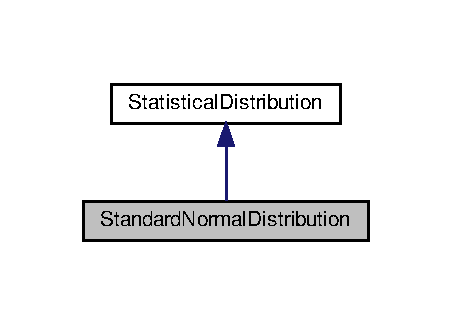
\includegraphics[width=217pt]{classStandardNormalDistribution__inherit__graph}
\end{center}
\end{figure}


Collaboration diagram for Standard\+Normal\+Distribution\+:
\nopagebreak
\begin{figure}[H]
\begin{center}
\leavevmode
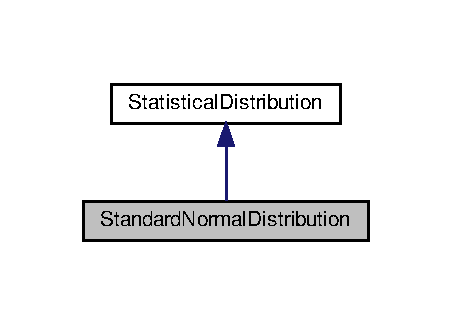
\includegraphics[width=217pt]{classStandardNormalDistribution__coll__graph}
\end{center}
\end{figure}
\subsection*{Public Member Functions}
\begin{DoxyCompactItemize}
\item 
\mbox{\Hypertarget{classStandardNormalDistribution_aa13a3e08de0d6c210f12f6b662a96797}\label{classStandardNormalDistribution_aa13a3e08de0d6c210f12f6b662a96797}} 
virtual double {\bfseries pdf} (const double \&x) const
\item 
\mbox{\Hypertarget{classStandardNormalDistribution_a3fa7f2413b10c05cbc9e08a96d4119cc}\label{classStandardNormalDistribution_a3fa7f2413b10c05cbc9e08a96d4119cc}} 
virtual double {\bfseries cdf} (const double \&x) const
\item 
\mbox{\Hypertarget{classStandardNormalDistribution_a51a7b166106a8d3a8cb49a6e39fede7e}\label{classStandardNormalDistribution_a51a7b166106a8d3a8cb49a6e39fede7e}} 
virtual double {\bfseries inv\+\_\+cdf} (const double \&quantile) const
\item 
\mbox{\Hypertarget{classStandardNormalDistribution_ac3a7c8dd5787428010756b1431904b53}\label{classStandardNormalDistribution_ac3a7c8dd5787428010756b1431904b53}} 
virtual double {\bfseries mean} () const
\item 
\mbox{\Hypertarget{classStandardNormalDistribution_a145bb7fff13e1daebaccd878c783ef1c}\label{classStandardNormalDistribution_a145bb7fff13e1daebaccd878c783ef1c}} 
virtual double \hyperlink{classStandardNormalDistribution_a145bb7fff13e1daebaccd878c783ef1c}{var} () const
\begin{DoxyCompactList}\small\item\em Equal to 0. \end{DoxyCompactList}\item 
\mbox{\Hypertarget{classStandardNormalDistribution_a453eee16a74d17e10fbdbf7c224d87d6}\label{classStandardNormalDistribution_a453eee16a74d17e10fbdbf7c224d87d6}} 
virtual double \hyperlink{classStandardNormalDistribution_a453eee16a74d17e10fbdbf7c224d87d6}{stddev} () const
\begin{DoxyCompactList}\small\item\em Equal to 1. \end{DoxyCompactList}\item 
\mbox{\Hypertarget{classStandardNormalDistribution_a5289fe3625483f32e0c82bafa467f20d}\label{classStandardNormalDistribution_a5289fe3625483f32e0c82bafa467f20d}} 
virtual void \hyperlink{classStandardNormalDistribution_a5289fe3625483f32e0c82bafa467f20d}{random\+\_\+draws} (const std\+::vector$<$ double $>$ \&uniform\+\_\+draws, std\+::vector$<$ double $>$ \&dist\+\_\+draws)
\begin{DoxyCompactList}\small\item\em Variable 1. \end{DoxyCompactList}\end{DoxyCompactItemize}


\subsection{Detailed Description}
Standard Normal Distribution Implementation. 

A more elaborate explanation here 

The documentation for this class was generated from the following files\+:\begin{DoxyCompactItemize}
\item 
/home/oohnohnoh1/\+Desktop/\+G\+I\+T/\+Research/\+Parallel/include/statistics.\+h\item 
/home/oohnohnoh1/\+Desktop/\+G\+I\+T/\+Research/\+Parallel/src/statistics.\+cxx\end{DoxyCompactItemize}

\hypertarget{classStatisticalDistribution}{}\section{Statistical\+Distribution Class Reference}
\label{classStatisticalDistribution}\index{Statistical\+Distribution@{Statistical\+Distribution}}
\subsection*{Public Member Functions}
\begin{DoxyCompactItemize}
\item 
\hyperlink{classStatisticalDistribution_a0c968a41a854b3d33310b7bd78a7238a}{Statistical\+Distribution} ()
\begin{DoxyCompactList}\small\item\em A constructor. \end{DoxyCompactList}\item 
virtual \hyperlink{classStatisticalDistribution_a0e7be123394637fb1bef9e7a23cc5618}{$\sim$\+Statistical\+Distribution} ()
\begin{DoxyCompactList}\small\item\em Virtual destructor. \end{DoxyCompactList}\item 
\mbox{\Hypertarget{classStatisticalDistribution_aef1b717d8c6bc58c5b5806d1b935eb12}\label{classStatisticalDistribution_aef1b717d8c6bc58c5b5806d1b935eb12}} 
virtual double {\bfseries pdf} (const double \&x) const =0
\item 
\mbox{\Hypertarget{classStatisticalDistribution_aa7f52f4c8cadc971d9e189453ea0eb95}\label{classStatisticalDistribution_aa7f52f4c8cadc971d9e189453ea0eb95}} 
virtual double {\bfseries cdf} (const double \&x) const =0
\item 
\mbox{\Hypertarget{classStatisticalDistribution_aff50a79b73032b6f63db797124ec310f}\label{classStatisticalDistribution_aff50a79b73032b6f63db797124ec310f}} 
virtual double {\bfseries inv\+\_\+cdf} (const double \&quantile) const =0
\item 
\mbox{\Hypertarget{classStatisticalDistribution_a68177d55b616f6c2f857ccf7afbf7789}\label{classStatisticalDistribution_a68177d55b616f6c2f857ccf7afbf7789}} 
virtual double {\bfseries mean} () const =0
\item 
\mbox{\Hypertarget{classStatisticalDistribution_ae66c6543b8d40d200b45d26f4fb3e3c2}\label{classStatisticalDistribution_ae66c6543b8d40d200b45d26f4fb3e3c2}} 
virtual double \hyperlink{classStatisticalDistribution_ae66c6543b8d40d200b45d26f4fb3e3c2}{var} () const =0
\begin{DoxyCompactList}\small\item\em Variable 1. \end{DoxyCompactList}\item 
\mbox{\Hypertarget{classStatisticalDistribution_af097e57c0d28489af68ca8a4edaebcac}\label{classStatisticalDistribution_af097e57c0d28489af68ca8a4edaebcac}} 
virtual double \hyperlink{classStatisticalDistribution_af097e57c0d28489af68ca8a4edaebcac}{stdev} () const =0
\begin{DoxyCompactList}\small\item\em Varable 2. \end{DoxyCompactList}\item 
\mbox{\Hypertarget{classStatisticalDistribution_affe04d41cb2e6f9526cc2ad4fb5fb150}\label{classStatisticalDistribution_affe04d41cb2e6f9526cc2ad4fb5fb150}} 
virtual void \hyperlink{classStatisticalDistribution_affe04d41cb2e6f9526cc2ad4fb5fb150}{random\+\_\+draws} (const std\+::vector$<$ double $>$ \&uniform\+\_\+draws, std\+::vector$<$ double $>$ \&dist\+\_\+draws)=0
\begin{DoxyCompactList}\small\item\em Variable 3. \end{DoxyCompactList}\end{DoxyCompactItemize}


\subsection{Constructor \& Destructor Documentation}
\mbox{\Hypertarget{classStatisticalDistribution_a0c968a41a854b3d33310b7bd78a7238a}\label{classStatisticalDistribution_a0c968a41a854b3d33310b7bd78a7238a}} 
\index{Statistical\+Distribution@{Statistical\+Distribution}!Statistical\+Distribution@{Statistical\+Distribution}}
\index{Statistical\+Distribution@{Statistical\+Distribution}!Statistical\+Distribution@{Statistical\+Distribution}}
\subsubsection{\texorpdfstring{Statistical\+Distribution()}{StatisticalDistribution()}}
{\footnotesize\ttfamily Statistical\+Distribution\+::\+Statistical\+Distribution (\begin{DoxyParamCaption}{ }\end{DoxyParamCaption})}



A constructor. 

Statistical Distribution constructor \mbox{\Hypertarget{classStatisticalDistribution_a0e7be123394637fb1bef9e7a23cc5618}\label{classStatisticalDistribution_a0e7be123394637fb1bef9e7a23cc5618}} 
\index{Statistical\+Distribution@{Statistical\+Distribution}!````~Statistical\+Distribution@{$\sim$\+Statistical\+Distribution}}
\index{````~Statistical\+Distribution@{$\sim$\+Statistical\+Distribution}!Statistical\+Distribution@{Statistical\+Distribution}}
\subsubsection{\texorpdfstring{$\sim$\+Statistical\+Distribution()}{~StatisticalDistribution()}}
{\footnotesize\ttfamily virtual Statistical\+Distribution\+::$\sim$\+Statistical\+Distribution (\begin{DoxyParamCaption}{ }\end{DoxyParamCaption})\hspace{0.3cm}{\ttfamily [virtual]}}



Virtual destructor. 

A more elaborate explanation here 

The documentation for this class was generated from the following file\+:\begin{DoxyCompactItemize}
\item 
/home/oohnohnoh1/\+Desktop/\+G\+I\+T/\+Research/\+Parallel/include/statistics.\+h\end{DoxyCompactItemize}

\hypertarget{classStr}{}\section{Str Class Reference}
\label{classStr}\index{Str@{Str}}


A constructor with a character pointer input.  




{\ttfamily \#include $<$openmp2.\+hpp$>$}

\subsection*{Public Types}
\begin{DoxyCompactItemize}
\item 
\mbox{\Hypertarget{classStr_a8a51ef48a27e5e597fde5edd7d36f7d8}\label{classStr_a8a51ef48a27e5e597fde5edd7d36f7d8}} 
typedef \hyperlink{classVec}{Vec}$<$ char $>$\+::size\+\_\+type {\bfseries size\+\_\+type}
\item 
\mbox{\Hypertarget{classStr_a8a51ef48a27e5e597fde5edd7d36f7d8}\label{classStr_a8a51ef48a27e5e597fde5edd7d36f7d8}} 
typedef \hyperlink{classVec}{Vec}$<$ char $>$\+::size\+\_\+type {\bfseries size\+\_\+type}
\end{DoxyCompactItemize}
\subsection*{Public Member Functions}
\begin{DoxyCompactItemize}
\item 
\mbox{\Hypertarget{classStr_afedfc049e090cc83be3ea834948f28ba}\label{classStr_afedfc049e090cc83be3ea834948f28ba}} 
{\bfseries Str} (size\+\_\+type n, char c)
\item 
\mbox{\Hypertarget{classStr_a8235816d2687bf223490568a18124cf4}\label{classStr_a8235816d2687bf223490568a18124cf4}} 
{\bfseries Str} (const char $\ast$cp)
\item 
\mbox{\Hypertarget{classStr_a92caed2384063dca67f93a9788ed1115}\label{classStr_a92caed2384063dca67f93a9788ed1115}} 
{\footnotesize template$<$class In $>$ }\\{\bfseries Str} (In b, In e)
\item 
\hyperlink{classStr_a51d07a34edbcb6ab60c23c0a1f6d2625}{Str} ()
\item 
\mbox{\Hypertarget{classStr_afedfc049e090cc83be3ea834948f28ba}\label{classStr_afedfc049e090cc83be3ea834948f28ba}} 
{\bfseries Str} (size\+\_\+type n, char c)
\item 
\hyperlink{classStr_a8235816d2687bf223490568a18124cf4}{Str} (const char $\ast$cp)
\begin{DoxyCompactList}\small\item\em A constructor with a character pointer input. \end{DoxyCompactList}\item 
\mbox{\Hypertarget{classStr_a92caed2384063dca67f93a9788ed1115}\label{classStr_a92caed2384063dca67f93a9788ed1115}} 
{\footnotesize template$<$class In $>$ }\\\hyperlink{classStr_a92caed2384063dca67f93a9788ed1115}{Str} (In b, In e)
\begin{DoxyCompactList}\small\item\em create a \hyperlink{classStr}{Str} from the range denoted by iterators b and e \end{DoxyCompactList}\end{DoxyCompactItemize}


\subsection{Detailed Description}
A constructor with a character pointer input. 



 \subsubsection*{Custom \hyperlink{classStr}{Str} class }

A numeric progression is a seuqence of numbers, where the value of each number depends on one or more of the previous value.

Objects of built-\/in types generally behave like values\+: Whenever we copy an object of such a type, the original and copy have the same value but are otherwise indepedent.

For most of the built-\/in types, the language also defines a rich set of operators and provides automatic conversions between logically similar types. For example, if we add an int and a double, the compiler automatically converts the int into a double

When we define our own classes, we control the extent to which the resulting objects behave like values. By defining copying and assigning appropriately, the class author an arrange for objects of that class to act like values -\/ that is, the class author can arrange for each object to have state that is independent of any other object.

Our \hyperlink{classVec}{Vec} and \hyperlink{classStudent__info}{Student\+\_\+info} classes are examples of types that act like values

We shall see that the class author an also control conversions and related operations on class objects, thereby providing classes whose objects behave even more similarly to objects of built-\/in types.

Defining a \hyperlink{classStr}{Str} class that lets us create objects that behave approproximately as we would like. 

\subsection{Constructor \& Destructor Documentation}
\mbox{\Hypertarget{classStr_a51d07a34edbcb6ab60c23c0a1f6d2625}\label{classStr_a51d07a34edbcb6ab60c23c0a1f6d2625}} 
\index{Str@{Str}!Str@{Str}}
\index{Str@{Str}!Str@{Str}}
\subsubsection{\texorpdfstring{Str()}{Str()}\hspace{0.1cm}{\footnotesize\ttfamily [1/2]}}
{\footnotesize\ttfamily Str\+::\+Str (\begin{DoxyParamCaption}{ }\end{DoxyParamCaption})\hspace{0.3cm}{\ttfamily [inline]}}

default constructor, create an empty str \mbox{\Hypertarget{classStr_a8235816d2687bf223490568a18124cf4}\label{classStr_a8235816d2687bf223490568a18124cf4}} 
\index{Str@{Str}!Str@{Str}}
\index{Str@{Str}!Str@{Str}}
\subsubsection{\texorpdfstring{Str()}{Str()}\hspace{0.1cm}{\footnotesize\ttfamily [2/2]}}
{\footnotesize\ttfamily Str\+::\+Str (\begin{DoxyParamCaption}\item[{const char $\ast$}]{cp }\end{DoxyParamCaption})\hspace{0.3cm}{\ttfamily [inline]}}



A constructor with a character pointer input. 

create a \hyperlink{classStr}{Str} containing n copies of c

Copy constructor 

The documentation for this class was generated from the following files\+:\begin{DoxyCompactItemize}
\item 
/home/oohnohnoh1/\+Desktop/\+G\+I\+T/\+Research/\+Parallel/src/openmp2.\+cxx\item 
/home/oohnohnoh1/\+Desktop/\+G\+I\+T/\+Research/\+Parallel/include/openmp2.\+hpp\end{DoxyCompactItemize}

\hypertarget{classStudent__info}{}\section{Student\+\_\+info Class Reference}
\label{classStudent__info}\index{Student\+\_\+info@{Student\+\_\+info}}
\subsection*{Public Member Functions}
\begin{DoxyCompactItemize}
\item 
\mbox{\Hypertarget{classStudent__info_a09c06b7959456c8f0f966aca0e937ba9}\label{classStudent__info_a09c06b7959456c8f0f966aca0e937ba9}} 
{\bfseries Student\+\_\+info} (std\+::istream \&is)
\item 
\mbox{\Hypertarget{classStudent__info_a5898dcdf6fa4b0a3fc47d84d9a0662c1}\label{classStudent__info_a5898dcdf6fa4b0a3fc47d84d9a0662c1}} 
{\bfseries Student\+\_\+info} (const \hyperlink{classStudent__info}{Student\+\_\+info} \&)
\item 
\mbox{\Hypertarget{classStudent__info_a3240356d42e140117ce99c238904ed88}\label{classStudent__info_a3240356d42e140117ce99c238904ed88}} 
\hyperlink{classStudent__info}{Student\+\_\+info} \& {\bfseries operator=} (const \hyperlink{classStudent__info}{Student\+\_\+info} \&)
\item 
\mbox{\Hypertarget{classStudent__info_aedf8317be1f5ba6f3747070f8753d5a0}\label{classStudent__info_aedf8317be1f5ba6f3747070f8753d5a0}} 
std\+::istream \& {\bfseries read} (std\+::istream \&)
\item 
\mbox{\Hypertarget{classStudent__info_a895ffb71a04a15baac6493bd70530d3f}\label{classStudent__info_a895ffb71a04a15baac6493bd70530d3f}} 
std\+::string {\bfseries name} () const
\item 
\mbox{\Hypertarget{classStudent__info_aa747a026fde190bcf679e57a492060b4}\label{classStudent__info_aa747a026fde190bcf679e57a492060b4}} 
double {\bfseries grade} () const
\end{DoxyCompactItemize}
\subsection*{Static Public Member Functions}
\begin{DoxyCompactItemize}
\item 
\mbox{\Hypertarget{classStudent__info_a4b7118b78d60f4d8a5c51b5ea1b94494}\label{classStudent__info_a4b7118b78d60f4d8a5c51b5ea1b94494}} 
static bool {\bfseries compare} (const \hyperlink{classStudent__info}{Student\+\_\+info} \&s1, const \hyperlink{classStudent__info}{Student\+\_\+info} \&s2)
\end{DoxyCompactItemize}


The documentation for this class was generated from the following files\+:\begin{DoxyCompactItemize}
\item 
/home/oohnohnoh1/\+Desktop/\+G\+I\+T/\+Research/\+Parallel/include/Student\+\_\+info.\+h\item 
/home/oohnohnoh1/\+Desktop/\+G\+I\+T/\+Research/\+Parallel/src/Student\+\_\+info.\+cc\item 
/home/oohnohnoh1/\+Desktop/\+G\+I\+T/\+Research/\+Parallel/src/Student\+\_\+info.\+cxx\end{DoxyCompactItemize}

\hypertarget{classSYN__Mat}{}\section{S\+Y\+N\+\_\+\+Mat$<$ T $>$ Class Template Reference}
\label{classSYN__Mat}\index{S\+Y\+N\+\_\+\+Mat$<$ T $>$@{S\+Y\+N\+\_\+\+Mat$<$ T $>$}}


Inheritance diagram for S\+Y\+N\+\_\+\+Mat$<$ T $>$\+:
\nopagebreak
\begin{figure}[H]
\begin{center}
\leavevmode
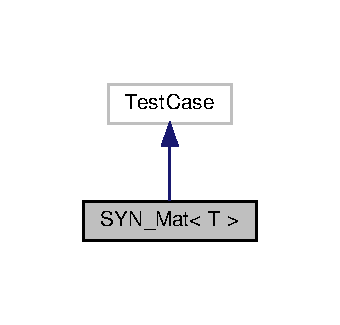
\includegraphics[width=163pt]{classSYN__Mat__inherit__graph}
\end{center}
\end{figure}


Collaboration diagram for S\+Y\+N\+\_\+\+Mat$<$ T $>$\+:
\nopagebreak
\begin{figure}[H]
\begin{center}
\leavevmode
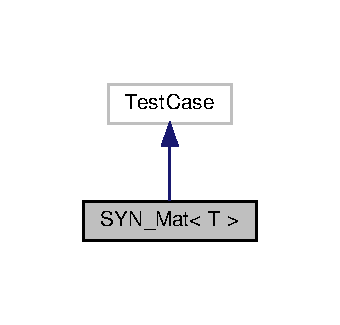
\includegraphics[width=163pt]{classSYN__Mat__coll__graph}
\end{center}
\end{figure}
\subsection*{Public Member Functions}
\begin{DoxyCompactItemize}
\item 
\mbox{\Hypertarget{classSYN__Mat_a81e0af5a7bd32ed70b44f319fc8edc39}\label{classSYN__Mat_a81e0af5a7bd32ed70b44f319fc8edc39}} 
{\bfseries S\+Y\+N\+\_\+\+Mat} (unsigned \+\_\+rows, unsigned \+\_\+cols, const T \&\+\_\+initial)
\item 
\mbox{\Hypertarget{classSYN__Mat_ab6ae892453033358fb394eb337f9722e}\label{classSYN__Mat_ab6ae892453033358fb394eb337f9722e}} 
{\bfseries S\+Y\+N\+\_\+\+Mat} (const \hyperlink{classSYN__Mat}{S\+Y\+N\+\_\+\+Mat}$<$ T $>$ \&alloc)
\item 
\mbox{\Hypertarget{classSYN__Mat_a8c26c6e94cafc98eabd4507859a8ef46}\label{classSYN__Mat_a8c26c6e94cafc98eabd4507859a8ef46}} 
\hyperlink{classSYN__Mat}{S\+Y\+N\+\_\+\+Mat}$<$ T $>$ \& {\bfseries operator=} (const \hyperlink{classSYN__Mat}{S\+Y\+N\+\_\+\+Mat}$<$ T $>$ \&alloc)
\item 
\mbox{\Hypertarget{classSYN__Mat_aab586b6842b14d810db853f0b44bb0d9}\label{classSYN__Mat_aab586b6842b14d810db853f0b44bb0d9}} 
\hyperlink{classSYN__Mat}{S\+Y\+N\+\_\+\+Mat}$<$ T $>$ {\bfseries operator+} (const \hyperlink{classSYN__Mat}{S\+Y\+N\+\_\+\+Mat}$<$ T $>$ \&rhs)
\item 
\mbox{\Hypertarget{classSYN__Mat_ab28a10ef6248599f000585dd1ac52f2b}\label{classSYN__Mat_ab28a10ef6248599f000585dd1ac52f2b}} 
\hyperlink{classSYN__Mat}{S\+Y\+N\+\_\+\+Mat}$<$ T $>$ \& {\bfseries operator+=} (const \hyperlink{classSYN__Mat}{S\+Y\+N\+\_\+\+Mat}$<$ T $>$ \&rhs)
\item 
\mbox{\Hypertarget{classSYN__Mat_a604d9395da807c16a38ee58ccbd9626a}\label{classSYN__Mat_a604d9395da807c16a38ee58ccbd9626a}} 
\hyperlink{classSYN__Mat}{S\+Y\+N\+\_\+\+Mat}$<$ T $>$ {\bfseries operator-\/} (const \hyperlink{classSYN__Mat}{S\+Y\+N\+\_\+\+Mat}$<$ T $>$ \&rhs)
\item 
\mbox{\Hypertarget{classSYN__Mat_a0e7915cbc22b0acf1050d98cbf1f8b9f}\label{classSYN__Mat_a0e7915cbc22b0acf1050d98cbf1f8b9f}} 
\hyperlink{classSYN__Mat}{S\+Y\+N\+\_\+\+Mat}$<$ T $>$ \& {\bfseries operator-\/=} (const \hyperlink{classSYN__Mat}{S\+Y\+N\+\_\+\+Mat}$<$ T $>$ \&rhs)
\item 
\mbox{\Hypertarget{classSYN__Mat_a9b84efa4ab4700395662c912592f140e}\label{classSYN__Mat_a9b84efa4ab4700395662c912592f140e}} 
\hyperlink{classSYN__Mat}{S\+Y\+N\+\_\+\+Mat}$<$ T $>$ {\bfseries operator$\ast$} (const \hyperlink{classSYN__Mat}{S\+Y\+N\+\_\+\+Mat}$<$ T $>$ \&rhs)
\item 
\mbox{\Hypertarget{classSYN__Mat_a4e7c3bf2add1eff8340bfb0ee370d9a7}\label{classSYN__Mat_a4e7c3bf2add1eff8340bfb0ee370d9a7}} 
\hyperlink{classSYN__Mat}{S\+Y\+N\+\_\+\+Mat}$<$ T $>$ \& {\bfseries operator$\ast$=} (const \hyperlink{classSYN__Mat}{S\+Y\+N\+\_\+\+Mat}$<$ T $>$ \&rhs)
\item 
\mbox{\Hypertarget{classSYN__Mat_ae7abe122e4fff8c1349092f1433b621a}\label{classSYN__Mat_ae7abe122e4fff8c1349092f1433b621a}} 
\hyperlink{classSYN__Mat}{S\+Y\+N\+\_\+\+Mat}$<$ T $>$ {\bfseries transpose} ()
\item 
\mbox{\Hypertarget{classSYN__Mat_a798ff5d5995916b0eb1f73beccfcd46b}\label{classSYN__Mat_a798ff5d5995916b0eb1f73beccfcd46b}} 
\hyperlink{classSYN__Mat}{S\+Y\+N\+\_\+\+Mat}$<$ T $>$ {\bfseries operator+} (const T \&rhs)
\item 
\mbox{\Hypertarget{classSYN__Mat_a144f03048627b72926ce073e1cf7a731}\label{classSYN__Mat_a144f03048627b72926ce073e1cf7a731}} 
\hyperlink{classSYN__Mat}{S\+Y\+N\+\_\+\+Mat}$<$ T $>$ {\bfseries operator-\/} (const T \&rhs)
\item 
\mbox{\Hypertarget{classSYN__Mat_aa6e7809760f004c41a7cf80459064788}\label{classSYN__Mat_aa6e7809760f004c41a7cf80459064788}} 
\hyperlink{classSYN__Mat}{S\+Y\+N\+\_\+\+Mat}$<$ T $>$ {\bfseries operator$\ast$} (const T \&rhs)
\item 
\mbox{\Hypertarget{classSYN__Mat_a7d70fe600d7bbe193c20162b3f0679fc}\label{classSYN__Mat_a7d70fe600d7bbe193c20162b3f0679fc}} 
\hyperlink{classSYN__Mat}{S\+Y\+N\+\_\+\+Mat}$<$ T $>$ {\bfseries operator/} (const T \&rhs)
\item 
\mbox{\Hypertarget{classSYN__Mat_a161e81b525a7f8dde96d071e21b21958}\label{classSYN__Mat_a161e81b525a7f8dde96d071e21b21958}} 
std\+::vector$<$ T $>$ {\bfseries operator$\ast$} (const std\+::vector$<$ T $>$ \&rhs)
\item 
\mbox{\Hypertarget{classSYN__Mat_a6e344855dbfa80bc534e04b1e66c90f5}\label{classSYN__Mat_a6e344855dbfa80bc534e04b1e66c90f5}} 
std\+::vector$<$ T $>$ {\bfseries diag\+\_\+vec} ()
\item 
\mbox{\Hypertarget{classSYN__Mat_ad9dd55a5a6c9151ee309940a693c7d1d}\label{classSYN__Mat_ad9dd55a5a6c9151ee309940a693c7d1d}} 
T \& {\bfseries operator()} (const unsigned \&row, const unsigned \&col)
\item 
\mbox{\Hypertarget{classSYN__Mat_ace7256e781e5dd3f71c53fb62f4c5fcd}\label{classSYN__Mat_ace7256e781e5dd3f71c53fb62f4c5fcd}} 
const T \& {\bfseries operator()} (const unsigned \&row, const unsigned \&col) const
\item 
\mbox{\Hypertarget{classSYN__Mat_af5ad6b2b5195b2b639699969ee2cdd8f}\label{classSYN__Mat_af5ad6b2b5195b2b639699969ee2cdd8f}} 
unsigned {\bfseries get\+\_\+rows} () const
\item 
\mbox{\Hypertarget{classSYN__Mat_a81c260deeb47134793364247264afc71}\label{classSYN__Mat_a81c260deeb47134793364247264afc71}} 
unsigned {\bfseries get\+\_\+cols} () const
\item 
\mbox{\Hypertarget{classSYN__Mat_afa91166dde91f354a19feb41517abee9}\label{classSYN__Mat_afa91166dde91f354a19feb41517abee9}} 
void {\bfseries test1} ()
\item 
\mbox{\Hypertarget{classSYN__Mat_a1d8c9032adf3c2aaf106081336a56950}\label{classSYN__Mat_a1d8c9032adf3c2aaf106081336a56950}} 
void {\bfseries test2} ()
\end{DoxyCompactItemize}


The documentation for this class was generated from the following files\+:\begin{DoxyCompactItemize}
\item 
/home/oohnohnoh1/\+Desktop/\+G\+I\+T/\+Research/\+Parallel/include/openmp\+\_\+\+L\+A.\+hpp\item 
/home/oohnohnoh1/\+Desktop/\+G\+I\+T/\+Research/\+Parallel/src/openmp\+\_\+\+L\+A.\+cxx\end{DoxyCompactItemize}

\hypertarget{classTemplateUnderTest}{}\section{Template\+Under\+Test$<$ T $>$ Class Template Reference}
\label{classTemplateUnderTest}\index{Template\+Under\+Test$<$ T $>$@{Template\+Under\+Test$<$ T $>$}}
\subsection*{Public Member Functions}
\begin{DoxyCompactItemize}
\item 
\mbox{\Hypertarget{classTemplateUnderTest_a4d1c3eb00df075511f89ec6e07b431ce}\label{classTemplateUnderTest_a4d1c3eb00df075511f89ec6e07b431ce}} 
{\bfseries Template\+Under\+Test} (T $\ast$t)
\item 
\mbox{\Hypertarget{classTemplateUnderTest_a31000e3b4f2738326708ffd1778a4fa1}\label{classTemplateUnderTest_a31000e3b4f2738326708ffd1778a4fa1}} 
void {\bfseries Some\+Method} ()
\end{DoxyCompactItemize}


The documentation for this class was generated from the following file\+:\begin{DoxyCompactItemize}
\item 
/home/oohnohnoh1/\+Desktop/\+G\+I\+T/\+Research/\+Parallel/include/openmp2.\+hpp\end{DoxyCompactItemize}

\hypertarget{classTrap}{}\section{Trap Class Reference}
\label{classTrap}\index{Trap@{Trap}}
\subsection*{Public Member Functions}
\begin{DoxyCompactItemize}
\item 
\mbox{\Hypertarget{classTrap_a510dd45e4b75d05c0af9ce21c1193999}\label{classTrap_a510dd45e4b75d05c0af9ce21c1193999}} 
void {\bfseries read} ()
\item 
\mbox{\Hypertarget{classTrap_af30bd4510371c688027c0a283f16b6e8}\label{classTrap_af30bd4510371c688027c0a283f16b6e8}} 
void {\bfseries compute\+Trapezium} ()
\end{DoxyCompactItemize}


The documentation for this class was generated from the following file\+:\begin{DoxyCompactItemize}
\item 
/home/oohnohnoh1/\+Desktop/\+G\+I\+T/\+Research/\+Parallel/include/trapezoid.\+hpp\end{DoxyCompactItemize}

\hypertarget{classVec}{}\section{Vec$<$ T $>$ Class Template Reference}
\label{classVec}\index{Vec$<$ T $>$@{Vec$<$ T $>$}}


Inheritance diagram for Vec$<$ T $>$\+:
\nopagebreak
\begin{figure}[H]
\begin{center}
\leavevmode
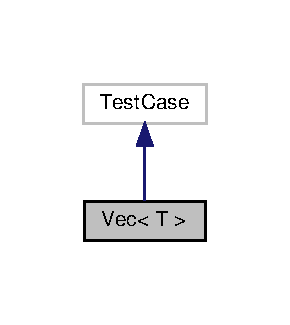
\includegraphics[width=139pt]{classVec__inherit__graph}
\end{center}
\end{figure}


Collaboration diagram for Vec$<$ T $>$\+:
\nopagebreak
\begin{figure}[H]
\begin{center}
\leavevmode
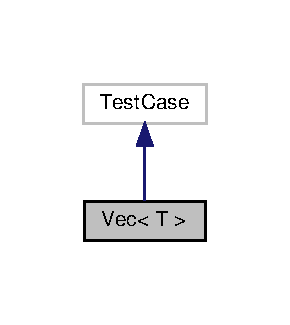
\includegraphics[width=139pt]{classVec__coll__graph}
\end{center}
\end{figure}
\subsection*{Public Types}
\begin{DoxyCompactItemize}
\item 
\mbox{\Hypertarget{classVec_a18d486e3211b998ce0dd000d95dddbbe}\label{classVec_a18d486e3211b998ce0dd000d95dddbbe}} 
typedef T $\ast$ {\bfseries iterator}
\item 
\mbox{\Hypertarget{classVec_a5208b137cec99b13ba74273cbdd564e4}\label{classVec_a5208b137cec99b13ba74273cbdd564e4}} 
typedef const T $\ast$ {\bfseries const\+\_\+iterator}
\item 
\mbox{\Hypertarget{classVec_aef386c702dd7e780c408c9cdb4cd0f40}\label{classVec_aef386c702dd7e780c408c9cdb4cd0f40}} 
typedef size\+\_\+t {\bfseries size\+\_\+type}
\item 
\mbox{\Hypertarget{classVec_a18d486e3211b998ce0dd000d95dddbbe}\label{classVec_a18d486e3211b998ce0dd000d95dddbbe}} 
typedef T $\ast$ {\bfseries iterator}
\item 
\mbox{\Hypertarget{classVec_a5208b137cec99b13ba74273cbdd564e4}\label{classVec_a5208b137cec99b13ba74273cbdd564e4}} 
typedef const T $\ast$ {\bfseries const\+\_\+iterator}
\item 
\mbox{\Hypertarget{classVec_aef386c702dd7e780c408c9cdb4cd0f40}\label{classVec_aef386c702dd7e780c408c9cdb4cd0f40}} 
typedef size\+\_\+t {\bfseries size\+\_\+type}
\item 
\mbox{\Hypertarget{classVec_a82bc529990b6ed767d347249381e6159}\label{classVec_a82bc529990b6ed767d347249381e6159}} 
typedef T {\bfseries value\+\_\+type}
\item 
\mbox{\Hypertarget{classVec_a604b2b35fed38bcf9d18a51fb5a673cc}\label{classVec_a604b2b35fed38bcf9d18a51fb5a673cc}} 
typedef T \& {\bfseries reference}
\item 
\mbox{\Hypertarget{classVec_a53eb22e4c8038c002212fef30490c109}\label{classVec_a53eb22e4c8038c002212fef30490c109}} 
typedef const T \& {\bfseries const\+\_\+reference}
\end{DoxyCompactItemize}
\subsection*{Public Member Functions}
\begin{DoxyCompactItemize}
\item 
\mbox{\Hypertarget{classVec_ac0a05e27809664ffb591f1c399ec1619}\label{classVec_ac0a05e27809664ffb591f1c399ec1619}} 
{\bfseries Vec} (size\+\_\+type n, const T \&t=T())
\item 
\mbox{\Hypertarget{classVec_a90bf23efb6803d9169953dc4d1b56279}\label{classVec_a90bf23efb6803d9169953dc4d1b56279}} 
{\bfseries Vec} (const \hyperlink{classVec}{Vec} \&v)
\item 
\mbox{\Hypertarget{classVec_a2f2d56035baaf1c59273ca133e9f0d92}\label{classVec_a2f2d56035baaf1c59273ca133e9f0d92}} 
\hyperlink{classVec}{Vec} \& {\bfseries operator=} (const \hyperlink{classVec}{Vec} \&)
\item 
\mbox{\Hypertarget{classVec_ad247d9fb26a955a24834396d89d17cdc}\label{classVec_ad247d9fb26a955a24834396d89d17cdc}} 
const T \& {\bfseries operator\mbox{[}$\,$\mbox{]}} (size\+\_\+type i) const
\item 
\mbox{\Hypertarget{classVec_a3eca41d5ac2286fa53786b60da27c6f1}\label{classVec_a3eca41d5ac2286fa53786b60da27c6f1}} 
void {\bfseries push\+\_\+back} (const T \&t)
\item 
\mbox{\Hypertarget{classVec_ae12d835a4e1789437cb38f78538e79c4}\label{classVec_ae12d835a4e1789437cb38f78538e79c4}} 
size\+\_\+type {\bfseries size} () const
\item 
\mbox{\Hypertarget{classVec_a4cc27fcb57f4f23c9eec6c88c71d5943}\label{classVec_a4cc27fcb57f4f23c9eec6c88c71d5943}} 
iterator {\bfseries begin} ()
\item 
\mbox{\Hypertarget{classVec_a7754cd19c8156677775ee13653460bbe}\label{classVec_a7754cd19c8156677775ee13653460bbe}} 
const\+\_\+iterator {\bfseries begin} () const
\item 
\mbox{\Hypertarget{classVec_a31cec2f83fbb4fcf6023b4eae8b03bab}\label{classVec_a31cec2f83fbb4fcf6023b4eae8b03bab}} 
iterator {\bfseries end} ()
\item 
\mbox{\Hypertarget{classVec_a151d00721f5f5668f4b37e408c2dc440}\label{classVec_a151d00721f5f5668f4b37e408c2dc440}} 
const\+\_\+iterator {\bfseries end} () const
\item 
\mbox{\Hypertarget{classVec_a8ceac4b6f24b88fbd768e185e10ac788}\label{classVec_a8ceac4b6f24b88fbd768e185e10ac788}} 
void {\bfseries run\+Test} ()
\end{DoxyCompactItemize}


The documentation for this class was generated from the following files\+:\begin{DoxyCompactItemize}
\item 
/home/oohnohnoh1/\+Desktop/\+G\+I\+T/\+Research/\+Parallel/include/M\+P\+I\+\_\+str.\+hpp\item 
/home/oohnohnoh1/\+Desktop/\+G\+I\+T/\+Research/\+Parallel/include/openmp1.\+hpp\end{DoxyCompactItemize}

\hypertarget{classtutorial_1_1Vec}{}\section{tutorial\+:\+:Vec$<$ T $>$ Class Template Reference}
\label{classtutorial_1_1Vec}\index{tutorial\+::\+Vec$<$ T $>$@{tutorial\+::\+Vec$<$ T $>$}}


The documentation for this class was generated from the following file\+:\begin{DoxyCompactItemize}
\item 
/home/oohnohnoh1/\+Desktop/\+G\+I\+T/\+Research/\+Parallel/include/lib\+\_\+mpi.\+hpp\end{DoxyCompactItemize}

\hypertarget{classVectorMethodTest}{}\section{Vector\+Method\+Test Class Reference}
\label{classVectorMethodTest}\index{Vector\+Method\+Test@{Vector\+Method\+Test}}


Inheritance diagram for Vector\+Method\+Test\+:\nopagebreak
\begin{figure}[H]
\begin{center}
\leavevmode
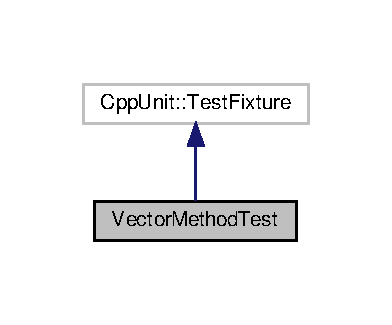
\includegraphics[width=188pt]{classVectorMethodTest__inherit__graph}
\end{center}
\end{figure}


Collaboration diagram for Vector\+Method\+Test\+:\nopagebreak
\begin{figure}[H]
\begin{center}
\leavevmode
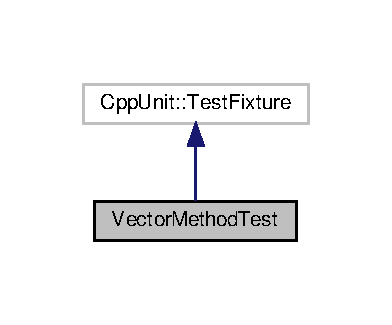
\includegraphics[width=188pt]{classVectorMethodTest__coll__graph}
\end{center}
\end{figure}
\subsection*{Public Member Functions}
\begin{DoxyCompactItemize}
\item 
\mbox{\Hypertarget{classVectorMethodTest_a4ca09c1329683bb368b6bd28df840f23}\label{classVectorMethodTest_a4ca09c1329683bb368b6bd28df840f23}} 
void {\bfseries set\+Up} ()
\item 
\mbox{\Hypertarget{classVectorMethodTest_a9a758704660f646ed8dfbc913dcb69f7}\label{classVectorMethodTest_a9a758704660f646ed8dfbc913dcb69f7}} 
void {\bfseries tear\+Down} ()
\item 
\mbox{\Hypertarget{classVectorMethodTest_aa81901684a9d920f34ebadfd0616c783}\label{classVectorMethodTest_aa81901684a9d920f34ebadfd0616c783}} 
void {\bfseries test\+Constructor} ()
\end{DoxyCompactItemize}


The documentation for this class was generated from the following file\+:\begin{DoxyCompactItemize}
\item 
/home/oohnohnoh1/\+Desktop/\+G\+I\+T/\+Research/\+Parallel/include/new.\+hpp\end{DoxyCompactItemize}

%--- End generated contents ---

% Index
\backmatter
\newpage
\phantomsection
\clearemptydoublepage
\addcontentsline{toc}{chapter}{Index}
\printindex

\end{document}
